\chapter{文獻回顧}







本研究探討的情境(參考\ref{chp:motivate})有以下需求:有易於拆裝的量測單位與被量測單位,能夠靈活應用於不同場域的三維相對定位。為滿足以上需求,需要有所需校正步驟少、體積小、能耗低、演算法簡單等特色。

在介紹本論文提出的定位方法之前,於\ref{chp:relative}先定義相對定位開始,依照\ref{pic:intro_pos}中的分類,依序介紹定位方法\ref{chp:method}與定位技術\ref{chp:technique},比較各自的優缺點,根據需求聚焦在「LED與PD定位技術」。\ref{chp:LEDandPD}便針對「LED與PD定位技術」進行深入探討,敘述此領域研究現況與困難。








% 重申自己主要的目標:(只有LED-PD近紅外光波段符合的原因)
% 低成本、不需預先了解環境資訊、裝設範圍小、方便架設、速度

\section{相對定位定義}
\label{chp:relative}
% -(利用數學符號描述相對定位問題的定義(軌跡、時間等))
    
    在開始進入文獻探討之前,需先以數學定義何謂本論文所欲量測之「相對定位」。我們將取得相對位置的一方稱為量測者,如案例中的機械手臂;而量測者所欲取得相對位置的特定物體稱為目標物,如案例中的移動載具;兩者皆為剛體。
    
    因此,可以將量測者與目標物各自視為兩移動座標系如圖\ref{pic:homo_trans},兩者在空間中各自有位置、旋轉的六個自由度,可以利用齊次座標轉換(Homogeneous Transformation)表示座標系之間的平移與旋轉(式\ref{eqn:homogeneous}),$^{PL}\boldsymbol{H}$表示將LED座標系上的點轉換至PD座標系上的齊次轉換矩陣,而$^{PL}\boldsymbol{T}$與$^{PL}\boldsymbol{Ro}$各自代表平移與旋轉的轉換矩陣,符號可參考符號列表(第\pageref{chp:symbol}頁)。
    
    \begin{figure}[ht]
        \centering
        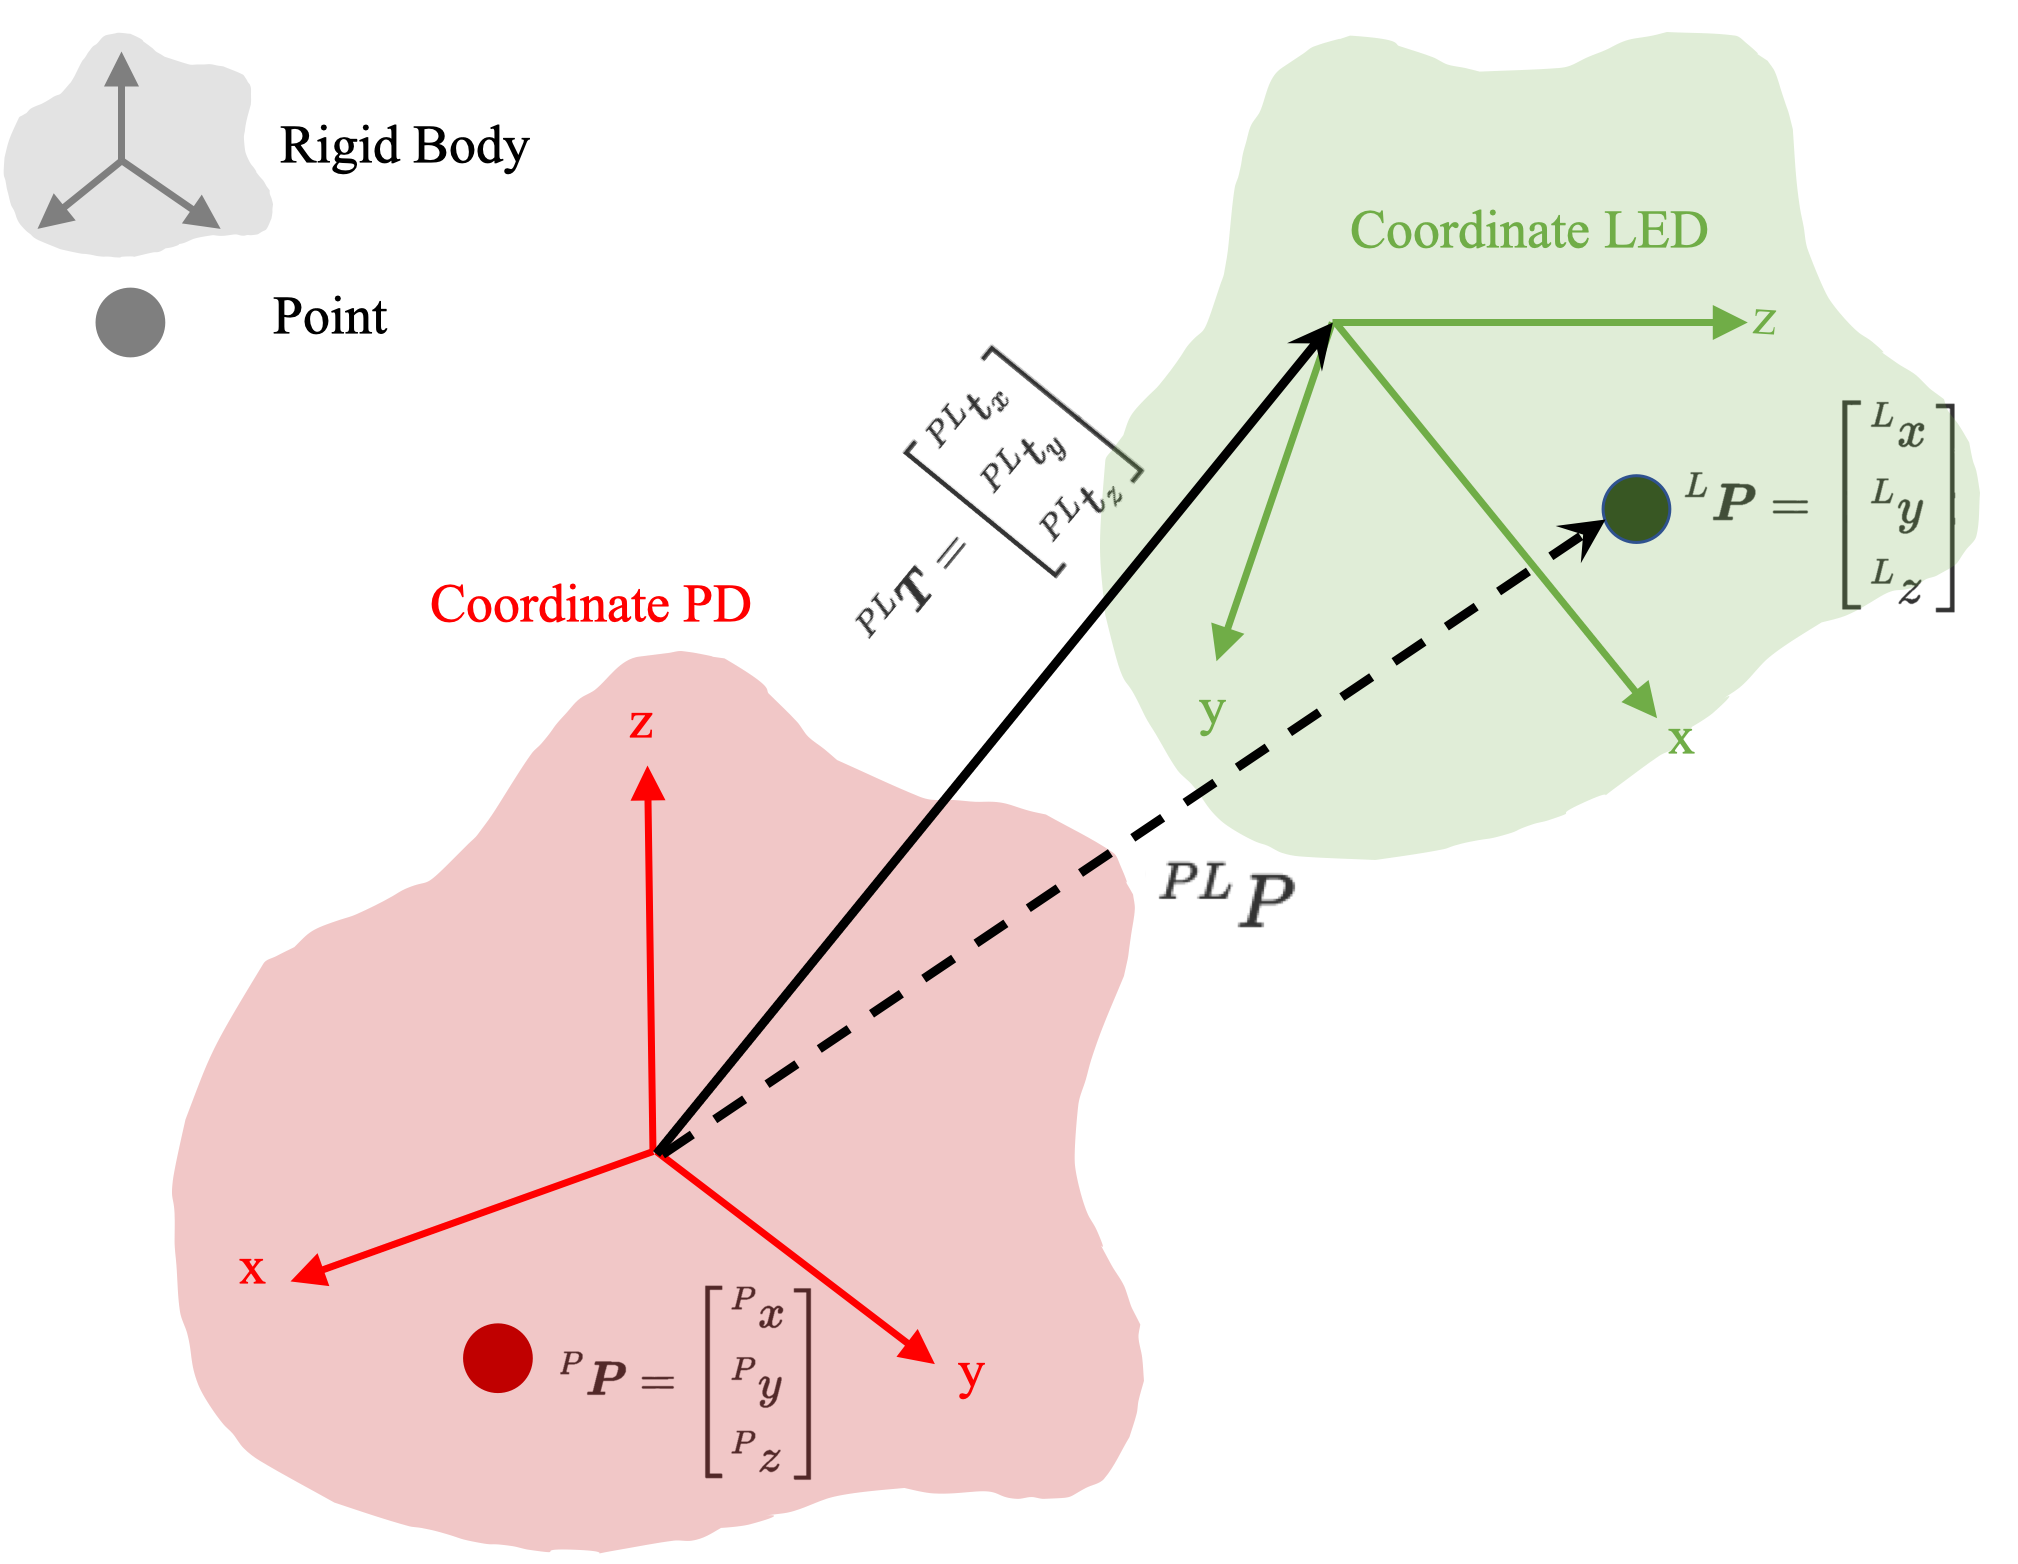
\includegraphics[width=9cm]{ch2pic/homo_trans.png}
        \caption{LED座標系與PD座標系及相對關係}
        \label{pic:homo_trans}
    \end{figure}

    \begin{equation}
        \label{eqn:homogeneous}
        \begin{aligned}
        {\left[\begin{array}{c}
        { }^{P L} P \\
        1
        \end{array}\right]={ }^{P L} \boldsymbol{H}\left[\begin{array}{c}
        { }^{L} P \\
        1
        \end{array}\right] } &=\left[\begin{array}{cc}
        { }^{P L} \boldsymbol{R} \boldsymbol{o} & { }^{P L} \boldsymbol{T} \\
        0 & 1
        \end{array}\right]\left[\begin{array}{c}
        { }^{L} P \\
        1
        \end{array}\right] \\
        &=\left[\begin{array}{cccc}
        { }^{P L} \gamma_{11} & { }^{P L} \gamma_{12} & { }^{P L} \gamma_{13} & { }^{P L} {t}_{x} \\
        { }^{P L} \gamma_{21} & ^{P L } \gamma_{22} & { }^{P L} \gamma_{23} & { }^{P L} {t}_{y} \\
        { }^{P L} \gamma_{31} & ^{P L} \gamma_{32} & { }^{P L} \gamma_{33} & { }^{P L} {t}_{z} \\
        0 & 0 & 0 & 1
        \end{array}\right]\left[\begin{array}{c}
        { }^{L} {x} \\
        { }^{L} {y} \\
        { }^{L} z \\
        1
        \end{array}\right]
        \end{aligned}
    \end{equation}

    % \begin{equation}
    %     ^{PL}\boldsymbol{T}=\left[\begin{array}{l}
    %     ^{PL}x \\ ^{PL}y \\ ^{PL}z
    %     \end{array}\right]
    % \end{equation}

    
    
   其中,兩座標系之間的平移關係$^{PL}\boldsymbol{T}$即為欲得到的相對位置資訊,共有三個自由度。

 



\section{後處理方法分類}
\label{chp:method}
    
    後處理方法可以分成兩部分:室內定位所使用的硬體在接收訊號時,首先會根據量測者所接收的資訊種類有所不同;接收資訊後,如何利用資訊計算出相對位置,則是屬於定位演算法的部分。
    
    

    \subsection{資訊種類}
    
    \begin{figure}[ht]
        \centering
        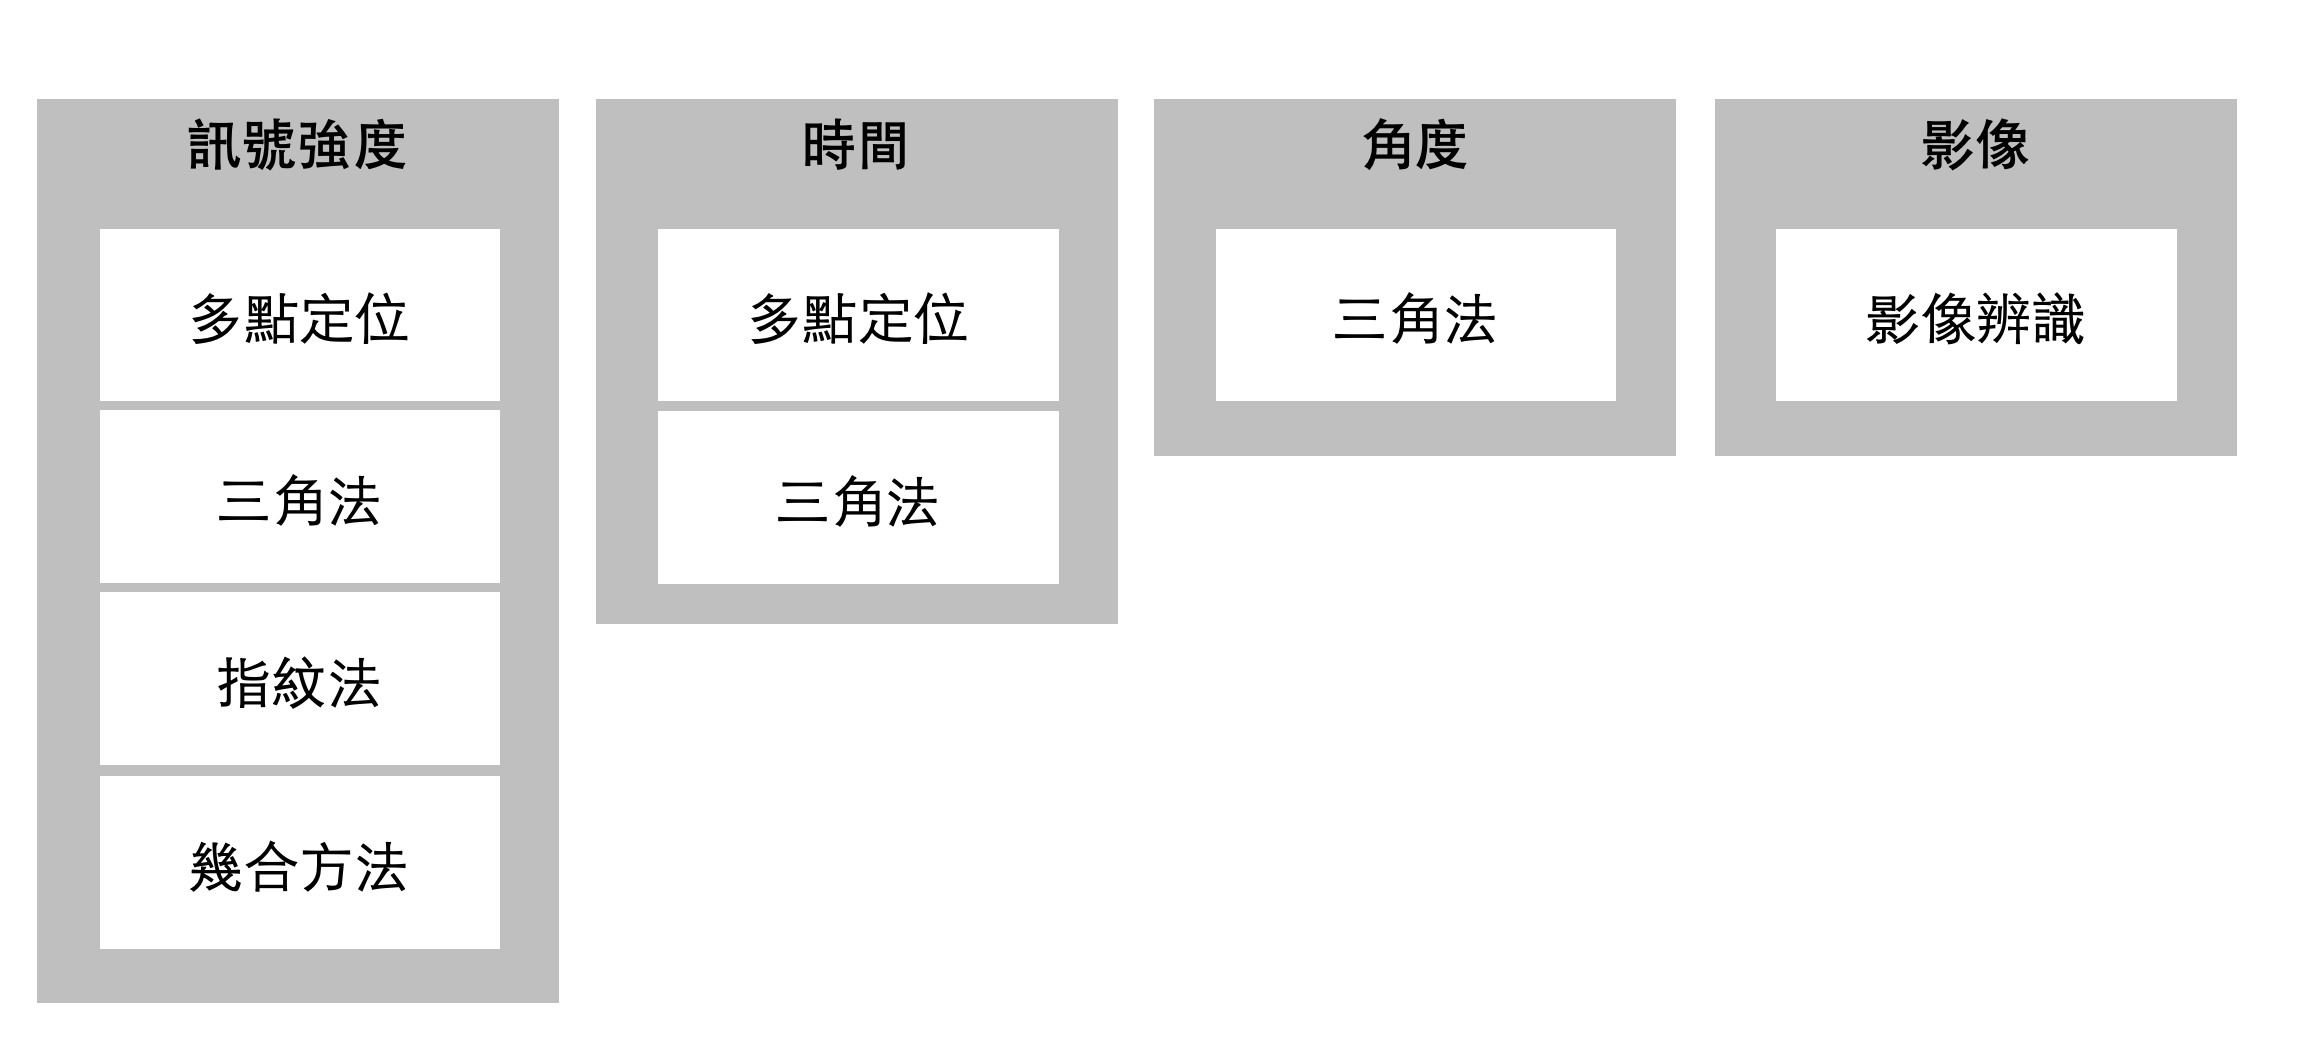
\includegraphics[width=12cm]{ch2pic/method_sort.png}
        \caption{資訊種類與演算法之間的關聯(參考\cite{survey_light2018})}
        \label{pic:method_sort}
    \end{figure}

    訊號強度(Received Signal Strength,簡寫RSS)為最常見的資訊種類,使用的是該硬體所接收到的訊號強度,而利用訊號強度的演算法也十分多樣,包含多點定位、三角法、指紋法等,可參考\ref{chp:method-algorithm}。

    時間資訊種類則是硬體利用訊號之間的時間差,量測距離的方法,常見使用的技術為紅外線,紅外線可以利用訊號傳送到不同接收子的時間差,判斷出之間的距離。若要利用時間資訊,在各硬體之間則需要將時間同步,在實作上為一大挑戰。

    若獲取的是角度資訊,基本上演算法便會搭配三角法,綜合多個接收子的角度獲得相對位置。

    影像則屬於相機獨有,且定位演算法為影像辨識,目標物需有已知的特徵,透過辨識影像中的特徵點,藉由特徵點於影像中呈現的大小、變形,進行計算以回推兩者之間的距離。


    \subsection{定位演算法}
    \label{chp:method-algorithm}
    常見的演算法種類如下:
    \begin{description}
        \item[- 多點定位(Multilateration)]\hfill 
        
        \qquad
        在環境中建立多個參考點並固定位置,利用目標物與多個參考點的距離,以各參考點為中心、距離為半徑畫圓求交點。
        \begin{figure}[ht]
            \centering
            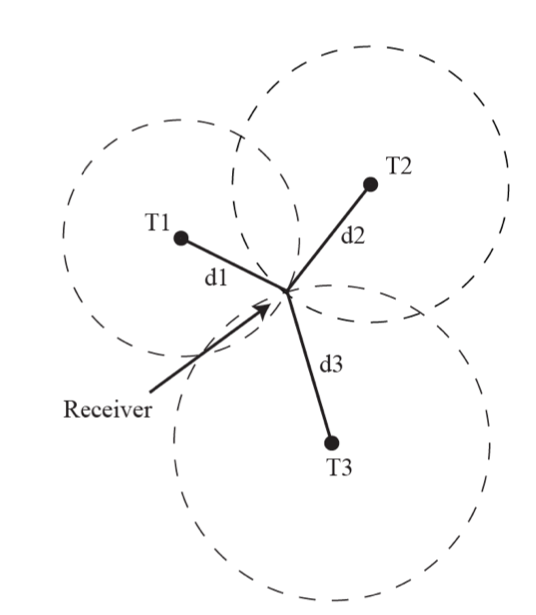
\includegraphics[width=6cm]{ch2pic/multilateration.png}
            \caption{多點定位法\cite{survey_light2020}}
            \label{pic:multilateration}
        \end{figure}
    
        \item[- 三角測量(Triangulation)] \hfill 
        
        \qquad
        在環境中建立多個參考點,藉由目標物與各參考點之間的角度關係,推算目標物位置。
        \begin{figure}[ht]
            \centering
            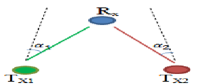
\includegraphics[width=4cm]{ch2pic/triangulation.png}
            \caption{三角測量法\cite{pic:triangulation}}
            \label{pic:triangulation}
        \end{figure}
        
        \item[- 指紋法(Fingerprinting)] \hfill 
        
        \qquad
        指紋法在環境中建立多個參考點,在實際進行測量前,需進行事先測量訓練的階段。在訓練階段時需將目標物在環境中移動,蒐集大量訊號數據庫,量測階段則藉由接收訊號與訓練階段所建立的數據庫參照,尋找最有可能存在的位置,近年則是有許多以機器學習方法增加此演算法的精確度。
        \begin{figure}[ht]
            \centering
            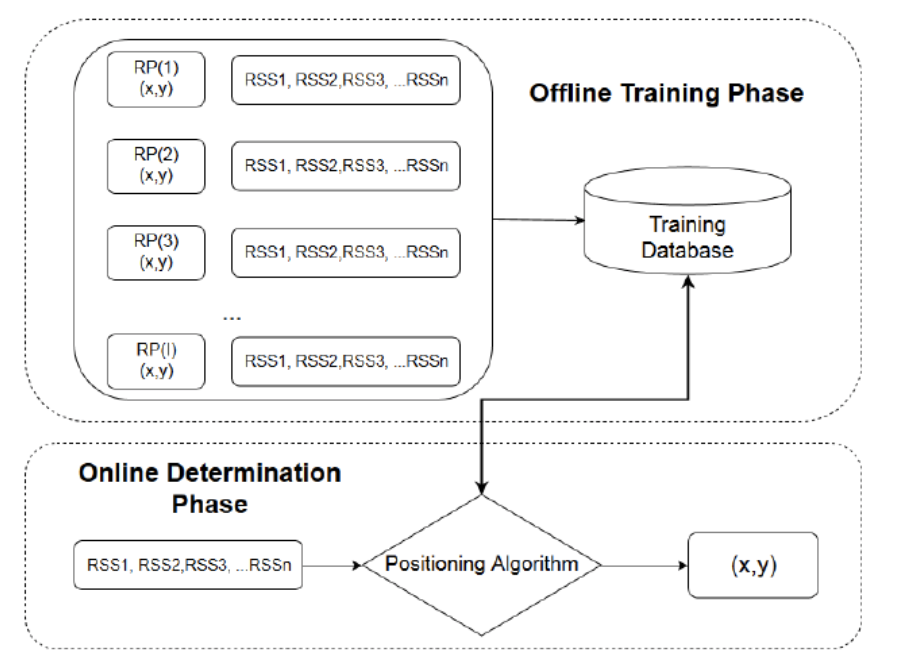
\includegraphics[width=13cm]{ch2pic/fingerprinting.png}
            \caption{指紋法流程圖\cite{pic:fingerprinting}}
            \label{pic:fingerprinting}
        \end{figure}
        
        \item[- 影像辨識]\hfill 
        
        \qquad
        三維空間中的物體,透過相機拍攝成為二維的影像時,為三維空間投影至二維影像平面上的幾何轉換。利用影像辨識求解相對位置時,則是試圖將二維影像中的特徵點比對、轉換回三維空間中,利用PnP演算法(Perspective-n-Point)解出目標物相對相機座標系的位置與方位。
        
        \begin{figure}[ht]
            \centering
            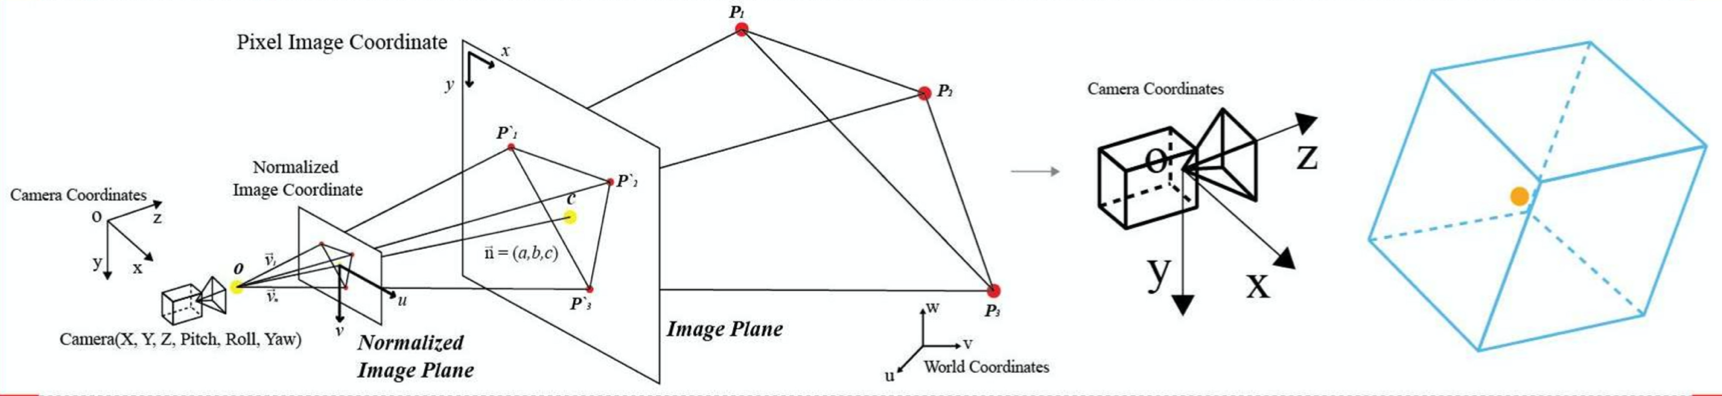
\includegraphics[width=15cm]{ch2pic/image_processing.png}
            \caption{影像辨識示意圖\cite{pic:image_processing}}
            \label{pic:image_processing}
        \end{figure}
        
        \qquad
        為了使辨識過程中,辨識特徵點的難度降低,通常會設計特徵明顯的標記,例如常見OpenCV中的ArUco標記,利用其快速的辨識ID以及距離、方位等資訊。
        
        \begin{figure}[ht]
            \centering
            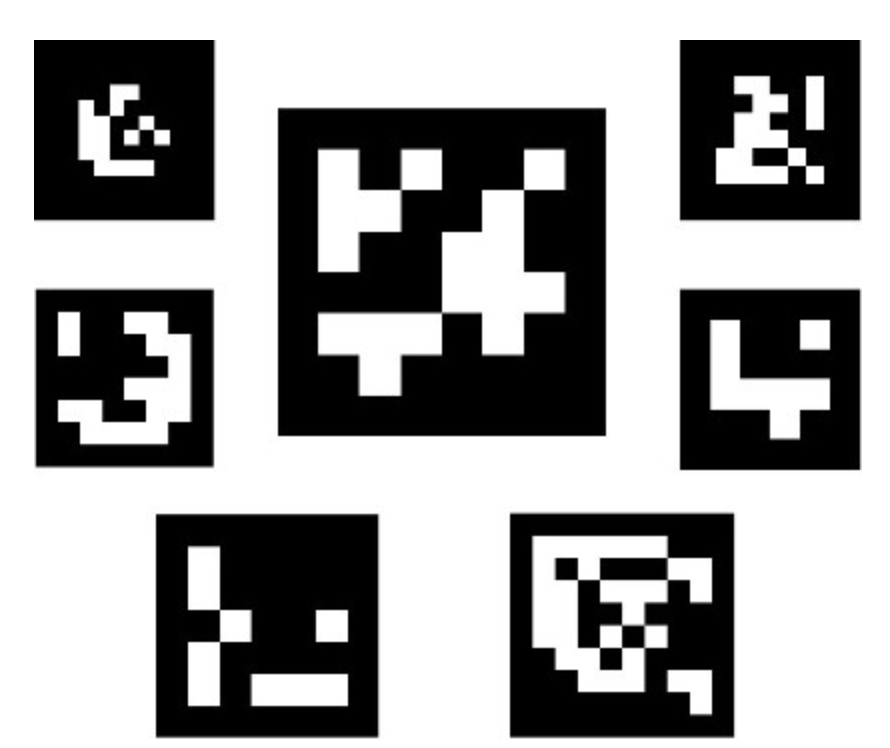
\includegraphics[width=5cm]{ch2pic/aruco.png}
            \caption{ArUco標記例子\cite{pic:aruco}}
            \label{pic:aruco}
        \end{figure}
        
        \item[- 幾何方法] \hfill 
        
        \qquad
        此類方法常見於LED與PD的定位方法,其接收的訊號強度與距離與角度皆有關,因此需綜合多點定位與三角定位,透過訊號強度與相對位置之間的幾何關係推算相對位置。
        
        \item[- 其他]\hfill 
        
        \qquad
        常見的其他種類演算法多會使用混合系統(Hybrid System),除了使用量測距離、角度等位置資訊的感測器,多與其他量測姿態、速度的感測器結合使用,如動作捕捉(Motion Capture)領域中使用慣性量測單元(Inertial Measurement Unit,簡稱IMU)量測點的移動軌跡。

    \end{description}

    \subsection{小結}

    根據\ref{chp:motivate}所總結對靈活度等的需求,演算法的影響較為顯著,而其中幾何方法是最合適的,因為此方法主要利用的為「兩者之間的幾何關係」,較能夠適應不同環境、不同擺放位置的改變,做到「一對一的定位」。相較起來,多點定位、三角法、指紋法都需要多個固定點的參考點的量測環境,無法符合易於安裝單元的需求,可以想像成「環境對一點的定位」。



\section{定位技術分類}
\label{chp:technique}

    室內定位所使用的技術(Technique)一樣十分多樣,非電磁波段的定位主要為超聲波,應用訊號發射與接收之間的時間差,推算與目標物之間的距離。然而該技術受溫度影響,且對目標物的辨識能力不佳,因此目前著重在自駕車與載具中障礙物的有無偵測上\cite{survey_ultrasonic},並不符合研究目標,所以以下章節聚焦在電磁波段內的定位進行分析。

    電磁波段內有許多不同現今受到關注的量測技術,電磁波段內常見的技術於\ref{chp:intro}內有簡單介紹,而電磁波以光速傳播,擁有高傳播速度與不受介質溫度與濕度影響的特性,減少可能對量測訊號造成影響的因素。

    \begin{figure}[ht]
        \centering
        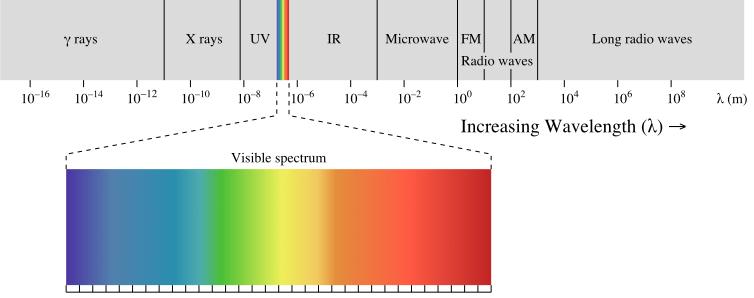
\includegraphics[width=12cm]{ch2pic/electro_spectrum.png}
        \caption{電磁波頻譜度\cite{Spectrum}}
        \label{pic:spectrum}
    \end{figure}

    我們由電磁波的頻率切入進行分類,頻譜圖如圖\ref{pic:spectrum},能夠用於定位的波段為頻率低於約790THz的波段,因為高於此波段的電磁波具有過高能量,電磁波頻率越高所含能量越高使高頻波段對人體有害,因此此波段中的X光、紫外線、伽瑪射線無法使用於日常應用,不予考慮。

    對人體無害的波段則分為兩部分探討:\ref{chp:radio}探討頻率低於300GHz的低頻波段\cite{book_electromagnetic},使用此波段的技術包含Wifi、藍芽、RFID;而在\ref{chp:light}介紹頻率介於790THz與300GHz之間的光波段,此波段的技術包含紅外線、可見光定位以及相機定位。以下章節便以圖\ref{pic:electro_sort}為架構依序介紹。


    \begin{figure}[ht]
        \centering
        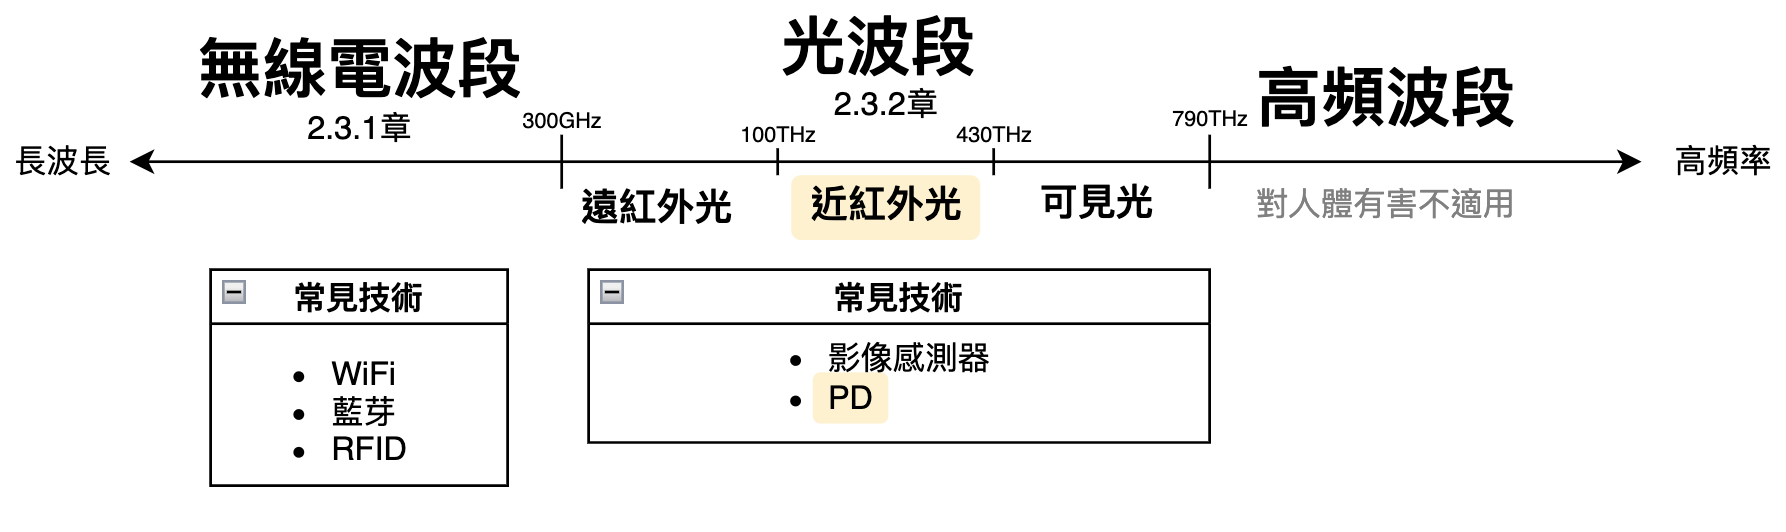
\includegraphics[width=13cm]{ch2pic/electro_sort.png}
        \caption{以電磁波頻率分類定位技術}
        \label{pic:electro_sort}
    \end{figure}

    











    \subsection{無線電波段定位}
    \label{chp:radio}
    
        低頻波段也就是俗稱的無線電波(Radio Waves),應用發展歷史長,對於可使用的頻率有嚴格規範,台灣由國家通訊委員會訂定嚴格的可使用頻率波段\cite{rf_law},保證軍警、醫療、廣播等的傳播需求。常見的定位技術包含室內與多數裝置既有的WiFi與藍芽裝置,或是較新的RFID定位技術。
    
        無線電波的主要特色包含可穿透大多障礙物,因此可用於跨房間非可視範圍(NLoS)的定位\cite{survey_indoor2018},增加了應用場域,然而也大大提升了訊號處理的難度,感測器難以辨別訊號衰減原因為距離、角度、亦或是障礙物,因此選擇非可視範圍內定位即捨棄精度。除此之外,無線電波的傳遞距離很長,定位範圍較廣,WiFi甚至可達距離50公尺的定位\cite{survey_indoor2014}。所需面對的誤差處理包含電磁干擾、同頻道干擾(Co-channel Interference)、受障礙物與金屬影響的穿透效果等。

        至於無線電波段所使用的定位演算法,大多系統皆是利用指紋法、多點定位、三角法的方式,共通點是都需要多個參考點,事先的安裝複雜,應用場域著重在固定場域,而精度多為公尺量級。
    
        舉例來說,此波段大多應用在固定的場域中,方法包含指紋法的建立數據庫,或是利用大量的感測器與訊號發射器來判斷定位\cite{survey_rfid},系統設置皆與圖\ref{pic:rfid_system}相似,差異於感測器擺放的方法以及演算法。其中,最經典的LANDMARC例子\cite{landmarc}的環境如圖\ref{pic:landmarc}所示,也是將感測器散布於環境中。

        

        \begin{figure}[ht]
            \centering
            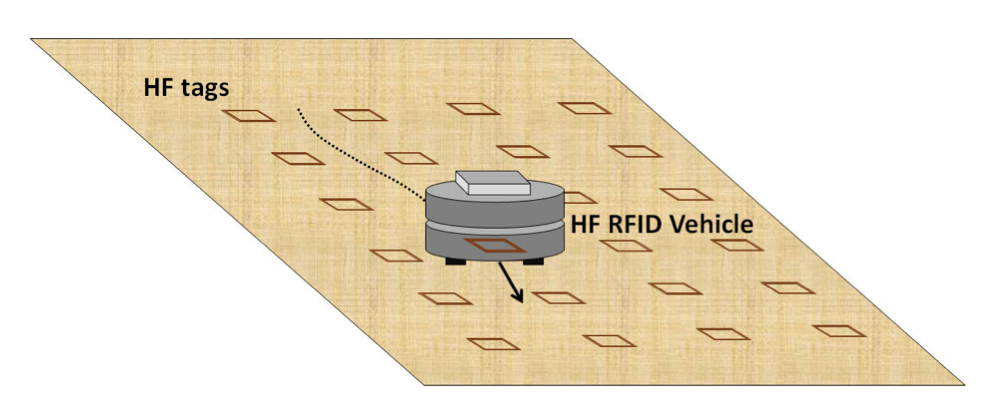
\includegraphics[width=6cm]{ch2pic/rfid_system.png}
            \caption{RFID定位系統示意\cite{survey_rfid}}
            \label{pic:rfid_system}
        \end{figure}

        \begin{figure}[ht]
            \centering
            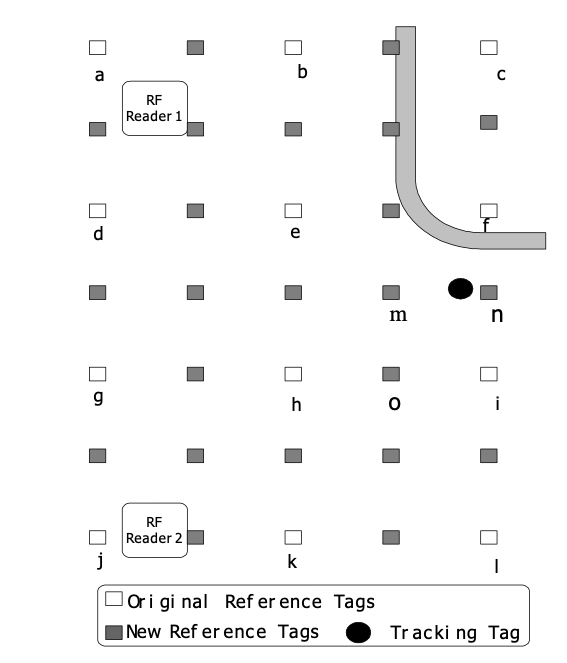
\includegraphics[width=8cm]{ch2pic/landmarc.png}
            \caption{LANDMARC系統\cite{landmarc}}
            \label{pic:landmarc}
        \end{figure}

        無線電波段也有少數例用\ref{chp:method-algorithm}中所提到的三角法,如\cite{case:rfid_1to1}研究(圖\ref{pic:rfid_1to1}),例用RFID天線所接收到的訊號強度與入射角度的關係,在載具上放置兩天線,而擺放角度有90度的差異,藉由RFID發射器傳送訊號至天線的入射角度不同,計算出目標物的方位。此文獻提出了一種一對一定位的方法,然而其只能解出目標物的方位,也就是二維定位中的角度,並不包含距離。除此之外,由於可穿透障礙物的特色,隨著測試環境中添加障礙物、人、移動物品,皆會影響到訊號,造成誤差。

        \begin{figure}[ht]
            \centering
            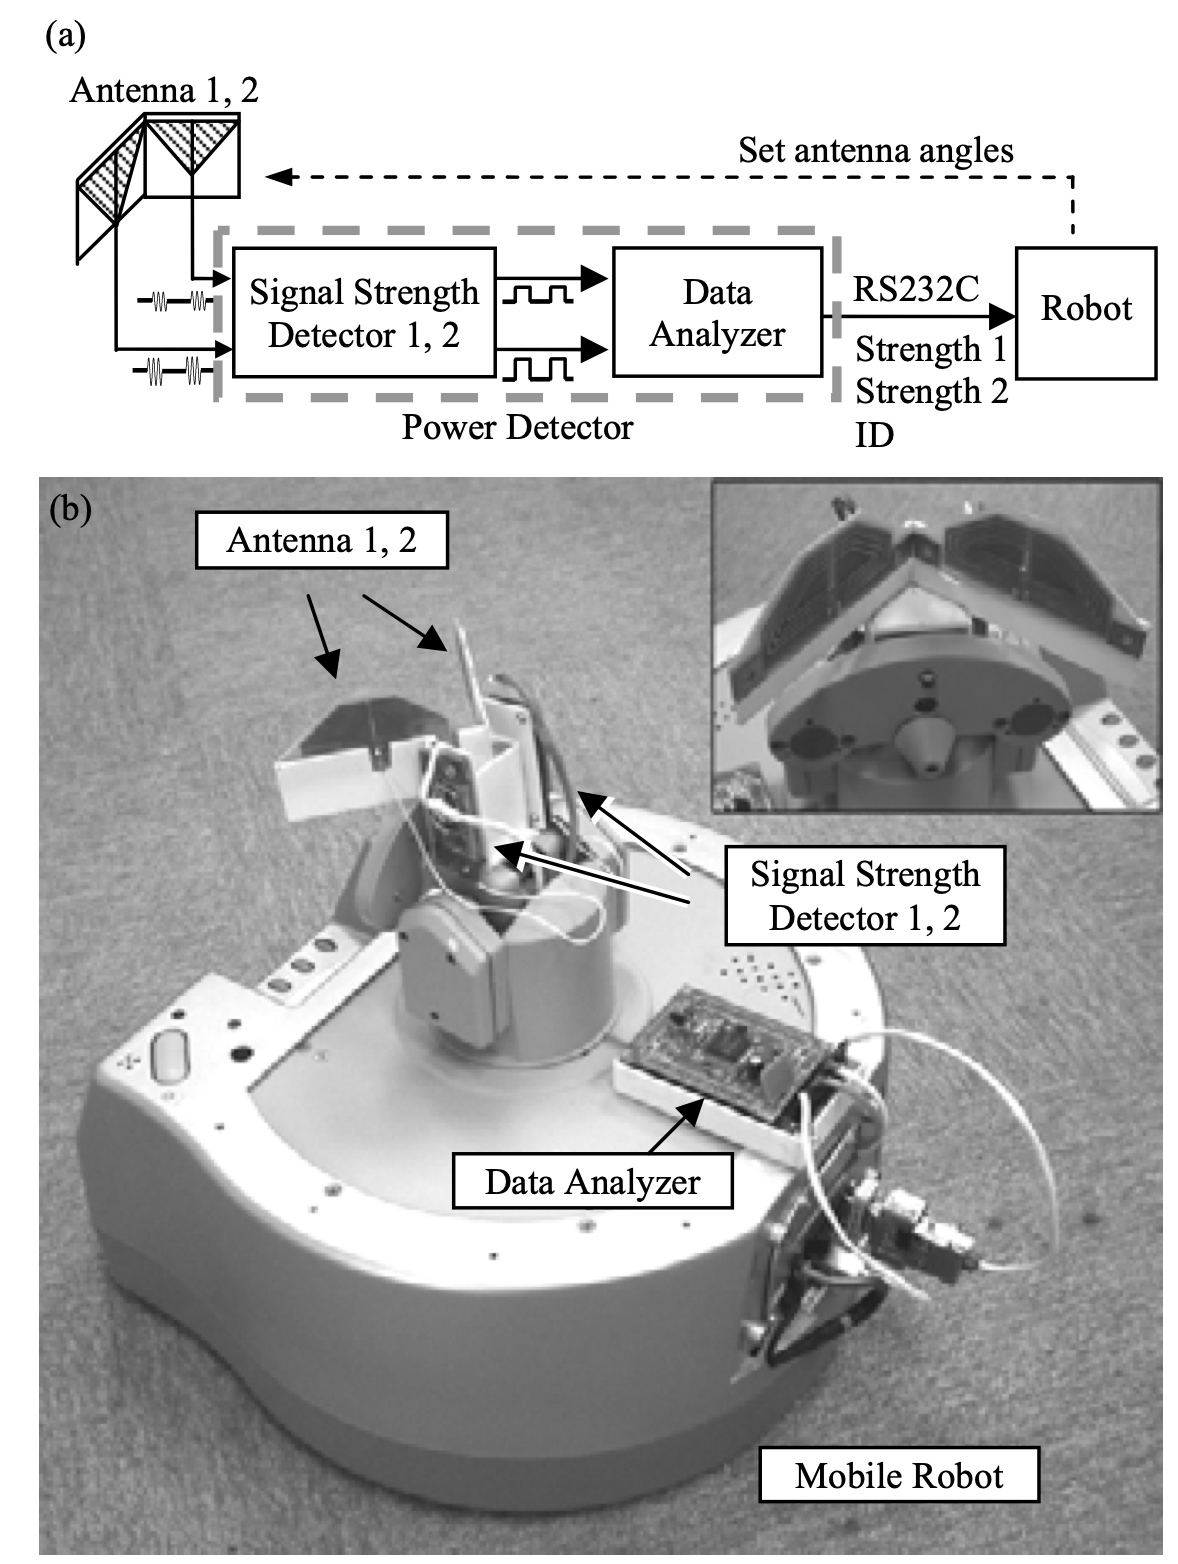
\includegraphics[width=8cm]{ch2pic/rfid_1to1.png}
            \caption{例用三角法定位的RFID系統\cite{case:rfid_1to1}(a)系統架構 (b)載具實驗}
            \label{pic:rfid_1to1}
        \end{figure}
        
        最後總結無線電波段的特色:此波段常使用於傳輸訊號的功能上,因此有成熟的編碼與解碼技術,能夠輕易達到辨識目標物的功能;而能夠穿透障礙物的特性,以及傳輸距離廣,使得應用範圍大又不受視線範圍拘束;然而精度相較低,因此大多仰賴多個參考點或是事前建立數據庫的指紋法,應用的靈活度降低,較不符合本研究目標,因此著重在\ref{chp:light}章中的光波段定位。

       



       


        \subsection{光波段定位}
        \label{chp:light}
            
            光波段的定位發展近幾年來十分顯著,主要原因為光學硬體上的進步,促使光通訊(Light Communication)的發展,使發光與感光元件具有傳播ID、訊息等資訊的能力,因此光通訊與光定位便於近年得到研究關注。光通訊流程如圖\ref{pic:vlc_flow}所示,利用驅動器調控光源的閃爍頻率、發光強度,來達到編碼的效果,最常見的編碼方式即為關閉調控(On-Off Keying,以下簡稱OOK),藉由開關光源傳送一段二進制訊號;感測器多以PD接收,接收後透過解碼取得資訊。

            \begin{figure}[ht]
                \centering
                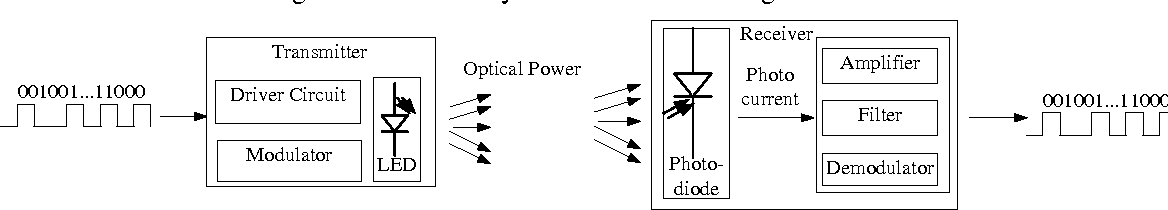
\includegraphics[width=15cm]{ch2pic/vlc_flow.png}
                \caption{光通訊流程圖\cite{pic:vlc}}
                \label{pic:vlc_flow}
            \end{figure}

            光波段在應用場域有一優勢,其可應用於於無線電波限制的場域,如機場與醫院等特殊醫療場域,在如今電磁波訊號充斥環境的狀況下,提供一替代方案。
            
            再來,光波段無法穿透障礙物,僅能進行可視範圍內(Line-of-Sight,以下簡稱LoS)的定位,捨棄廣域的定位,獲得較為單純的量測數據。此特性同時增加光通訊的安全性以及穩定度,著重針對可視範圍進行通訊與定位,不必考量其他訊號。例如載具運行時,僅需著重分析於身旁的其他物體,位於隔壁房間的物體毫不重要,因此可忽略不重要的資訊,增加處理速度與有用訊號穩定度。即便如此,僅能進行LoS定位也限制了能夠量測的範圍,在環境阻擋物較為複雜的環境會擋住光訊號的傳輸,使其無法進行定位。


            除此之外,電磁波有一特性為:波長愈短可達到的量測精度愈高,且感測器與訊號發射器的硬體大小也愈小,例如市售便宜常見的光波段感測器如PD感光二極體尺寸量級為mm或以下\cite{datasheet:led_sfh4545}且能耗低,而使用低頻波段的RFID感測器常見量級為cm\cite{datasheet:rfid_tag}。因此,選擇波長較短的光波段相較無線電波段具有硬體上的優勢。

            \begin{figure}[ht]
                \centering
                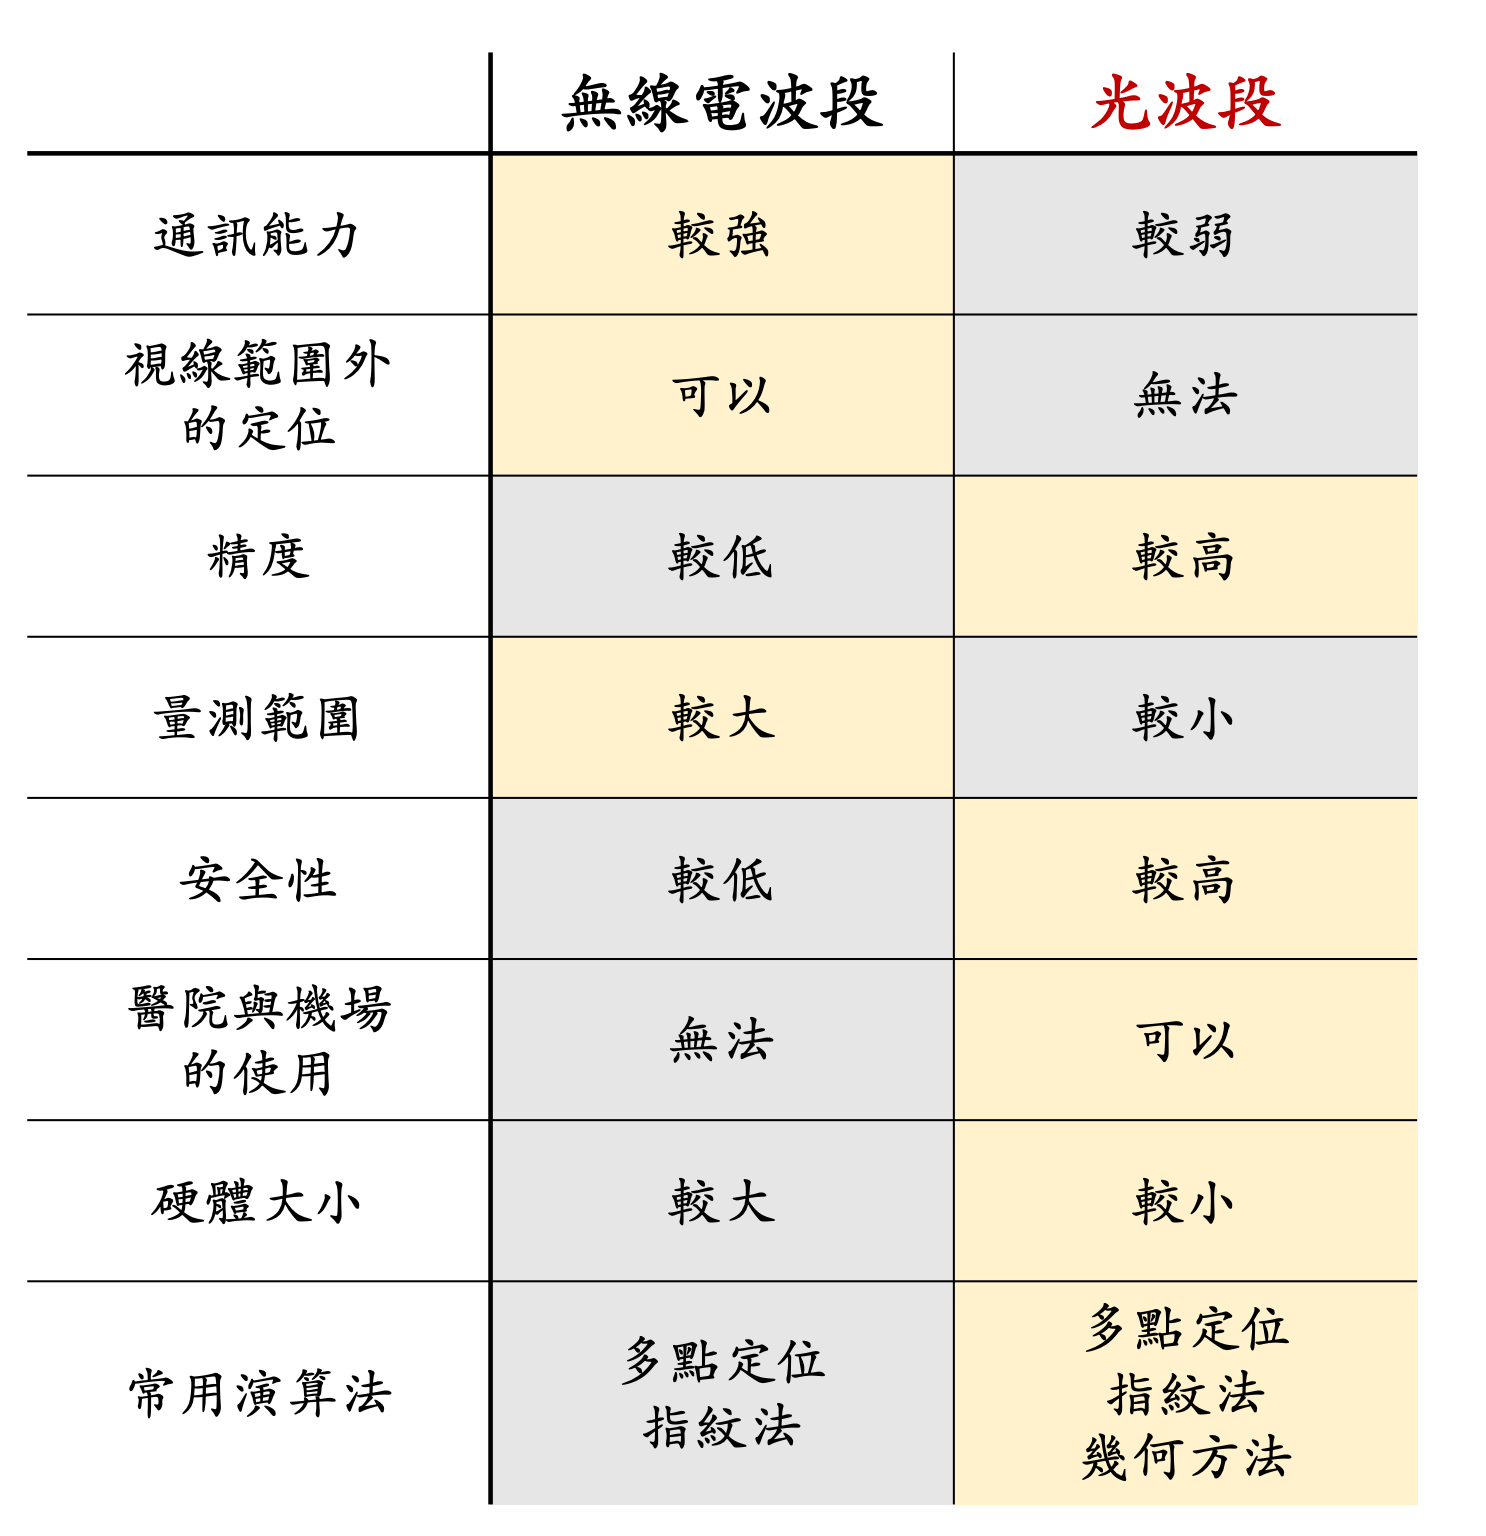
\includegraphics[width=12cm]{ch2pic/method_compare.png}
                \caption{無線電波段與光波段的比較}
                \label{pic:method_compare}
            \end{figure}


            光波段定位也分為許多種類(參考圖\ref{pic:electro_sort}),以下分別於\ref{chp:light_electro}探討使用波段的差異,以及於\ref{chp:light_receiver}介紹感測器硬體技術的選擇。


            \subsubsection{波段分類}

            \label{chp:light_electro}

            參考圖\ref{pic:electro_sort},光波段依照人眼可視與否分成可見光與紅外光兩類,而其中紅外光內由於硬體特性不同,又分為近紅外光與遠紅外光。以下依照不同面向條列討論:

            \begin{description}

                \item[- 人眼可視與否]\hfill 
                
                \qquad
                依照人眼可視區分為可見光與紅外光波段,而紅外光頻率低、能量較小,且於視網膜成像的難度也大,因此較為安全。而可見光的優勢於其可以照明,因此大多可見光定位會應用於需照明的場域,配合照明用的光線進行定位。但凡使用情境不想影響人們的感知,亦或是光源需移動,有直射眼境造成人眼不適的可能時,便會選擇使用紅外光波段。

                \qquad 
                本研究目標需應用於移動物體上,因此紅外光呈現優勢,紅外光無法在視網膜成像的特性讓使用者並不會感受到不適

                \item[- 成本] \hfill 
                
                \qquad
                光波段的光感測器常見的材料有矽(Si)、鍺(Ge)與III或V族元素,價格最便宜的是矽材料,而矽感測器的感光波段約在400-1000nm,也就是可見光與近紅外光(NIR)波段。但凡波長較長的紅外光在硬體材料便需要使用到昂貴的鍺或其他三五族元素\cite{si_pd},這也是為什麼普遍紅外光波段的硬體的印象都較為昂貴,然而近紅外光波段的感測器與可見光價格接近。

                \qquad
                除了硬體本身的成本以外,系統架設難易度也需納入考量。常見可見光定位的文獻會強調系統架設難易度低,因為可以利用室內常見的照明光源,不需額外添置訊號發射器。然而需注意的是,可見光定位需利用光通訊分辨ID時,進行編碼需要在光源硬體加裝驅動器,即代表需要將原有燈具改成能夠進行編碼的硬體、加裝驅動器等,所需付出的成本不得被忽視。因此,在架設成本上,我認為波段的無論影響不大。
                
                \qquad
                因此,僅考量成本時,無論是PD還是影像感測器,挑選可見光與近紅外光波段較為合適。
        
                \item[- 環境光源的影響] \hfill 
                
                \qquad
                光波段的誤差來源主要包含多重路徑傳輸(Multipath effect)與環境光源(Ambious Light Source)\cite{survey_light2020},其中多路徑傳輸無關波段,影響程度皆相同。而環境光源的部分,強度過高可造成訊號偏移,甚至硬體飽和導致訊號失真,因此需有效的降低環境光源的強度以保持定位的準確度。
            

                \qquad
                環境光源包含了室內的光源以及太陽光源,室內的光源使用交流電的頻率約在120hz,可以針對頻率進行濾波。而太陽光源的強度與電磁波頻率有關,可以由太陽輻射波譜(Solar Irradiance Spectrum)觀察強度與波長的關係。太陽光照射至地球時,傳送至地表的能量與大氣層的吸收度有關,高峰即為可見光波段,低谷則出現在760nm左右的氧氣吸收帶(Oxygen A-band)、與940nm和1550nm附近被水蒸氣吸收之波段\cite{book:solar_spectrum}。
                
                \begin{figure}[ht]
                    \centering
                    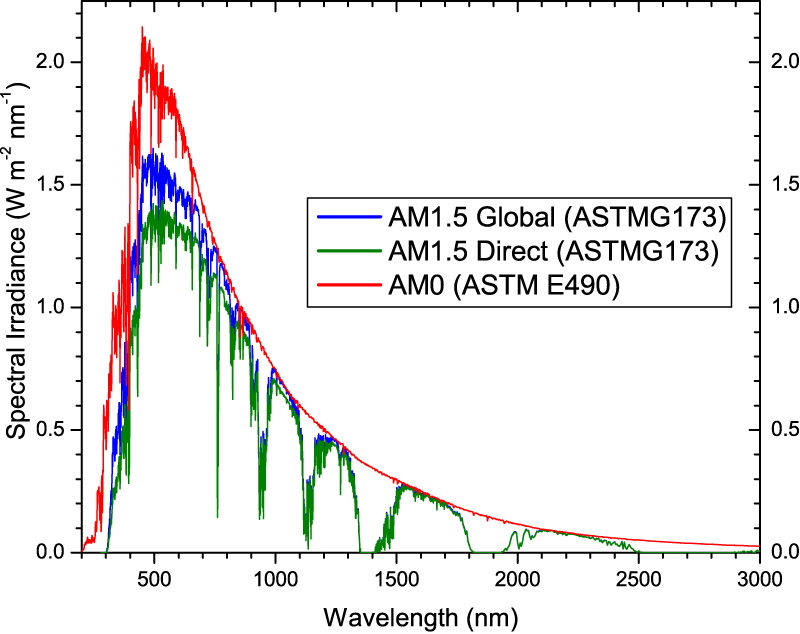
\includegraphics[width=10cm]{ch2pic/solar_spectra.png}
                    \caption{太陽輻射波譜\cite{astm}}
                    \label{pic:solar_spectrum}
                \end{figure}

                \qquad
                由於利用光波段定位最大誤差來源之一就是要克服其他光所造成的雜訊,因此在選擇工作波長時,需挑選太陽光能量較低的波段,也就是於近紅外光波段中的760nm與940nm,以及遠紅外光波段內的1550nm。
        
                \end{description}
                



                綜上所述,根據本研究的需求,最適合選擇使用近紅外光波段中的太陽能量低谷波段,簡單整理於圖\ref{pic:light_freq_compare},可以同時節省硬體成本、降低環境光源的影響,也能夠不造成使用者的眼經不適。

                \begin{figure}[ht]
                    \centering
                    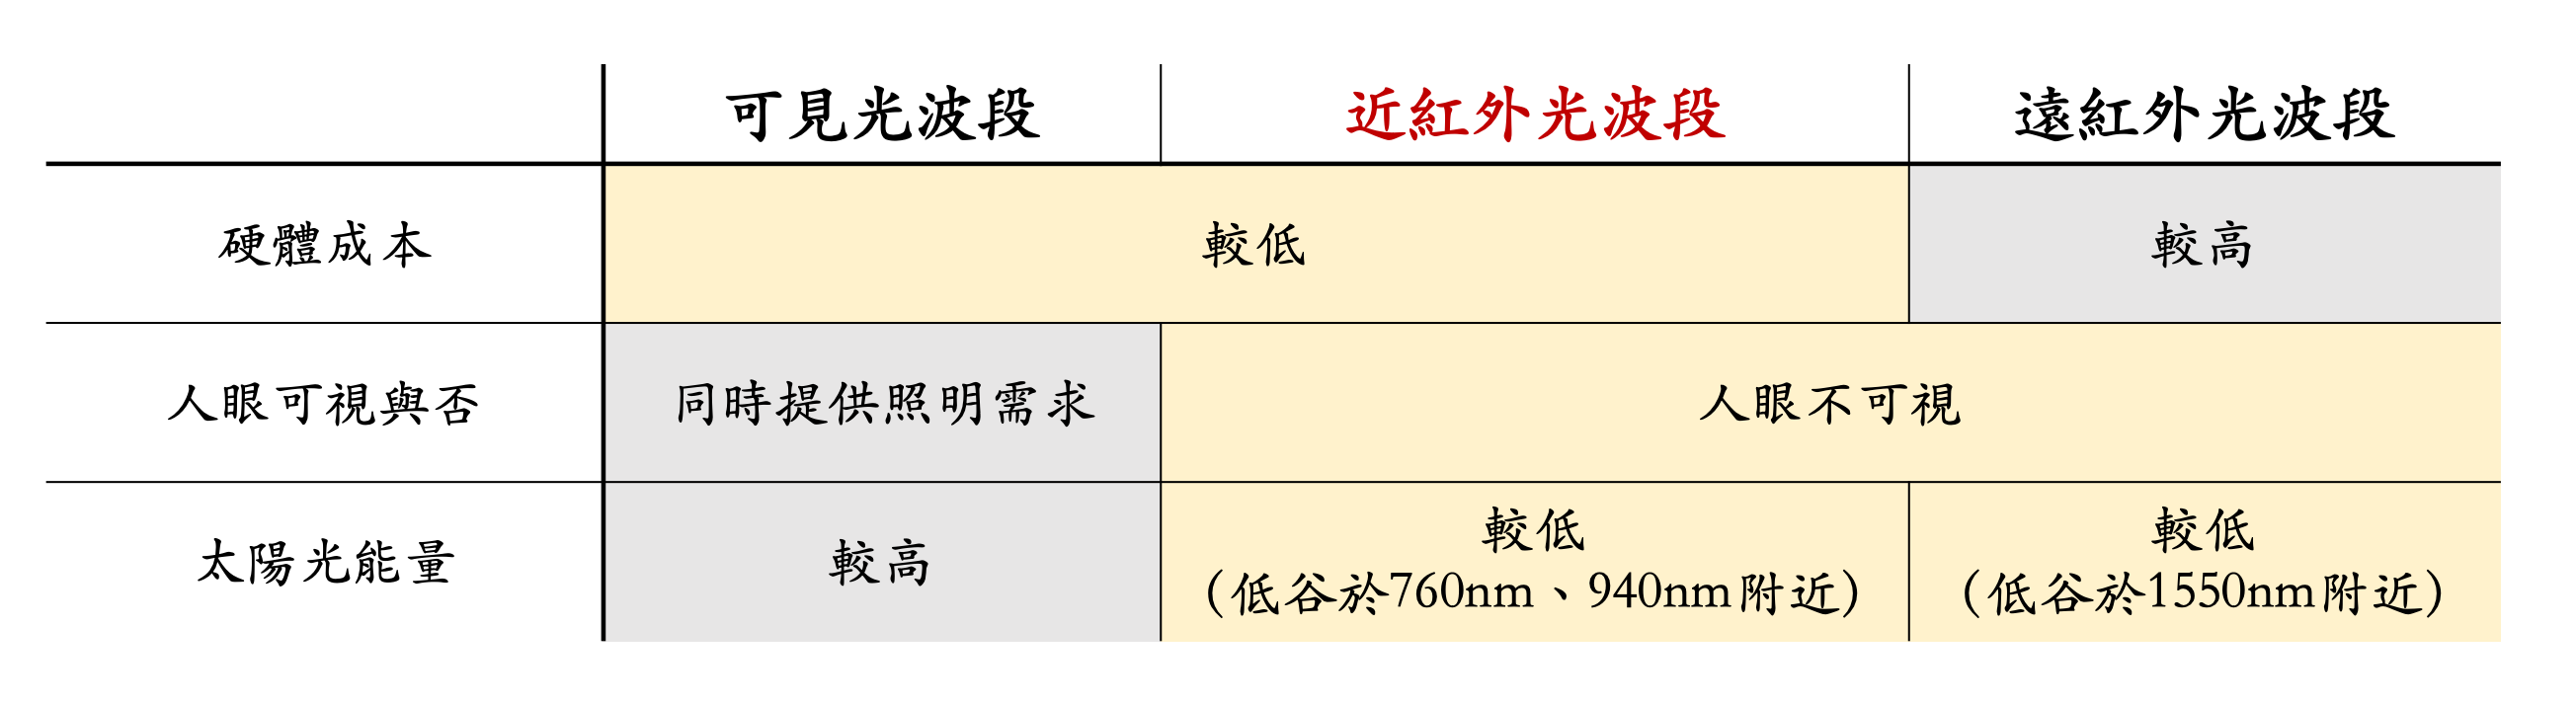
\includegraphics[width=15cm]{ch2pic/light_freq_compare.png}
                    \caption{光波段中的波段特性比較}
                    \label{pic:light_freq_compare}
                \end{figure}


            \subsubsection{接收子類型:PD與影像感測器}
            \label{chp:light_receiver}

                

                \ref{chp:light_electro}章中討論了光波段中不同波段的優缺點,而本小節中將討論光波段中常使用的兩種硬體差別,其分別為PD與影像感測器。

                \begin{description}

                    \item[- 影像感測器]\hfill 
                    
                    \qquad
                    影像感測器包含常見的相機,運作原理為每次取樣時,獲得多個像素的強度資訊,資訊量極多,是眾多定位技術中最消耗運算資源的。其定位方式是利用辨識已知的特徵圖案,進而將圖片中圖案的大小與變形與特徵進行比對,利用PnP眼算法推算目標物的距離以及姿態(參考\ref{chp:method-algorithm}章)。其中,若量測範圍要廣,由於隨距離增加,投射於影像平面上的圖案大小衰減快速,因此特徵圖案則需要越大越好。然而其取樣頻率大多在百赫茲內,且視覺辨識所需要的運算資源多,因此成本高,且運算速度也較慢。

                    \qquad
                    影像感測器所辨識的特徵點又可分為主動與被動傳送訊號的,被動傳送訊號的包含ArUco標誌(參考圖\ref{pic:aruco}),其需透過環境光源照設可見光波,讓影像感測器得以看到標誌,若室內光源未開,則無法定位。反之,主動傳送訊號的標誌便是光源,大多室內定位會使用半徑15公分以上的崁燈,利用相機的滾動式快門效應(Rolling Shutter Effect),將條紋圖案視為特徵辨識。其中,滾動式快門效應會造成條紋圖樣的原因可參考圖\ref{pic:rolling_shutter},因為CMOS感測器並非同時進行所有像素的成像,而是輪流一列一列的成像,搭配光源的閃爍,各列成像時便會各自呈現亮暗,因此產生條紋樣式。除此之外,透過調整光源的閃爍頻率,可以調整條紋的粗細,進而達到編碼與解碼的效果,如圖\ref{pic:rolling_shutter_case}。

                    \begin{figure}[ht]
                        \centering
                        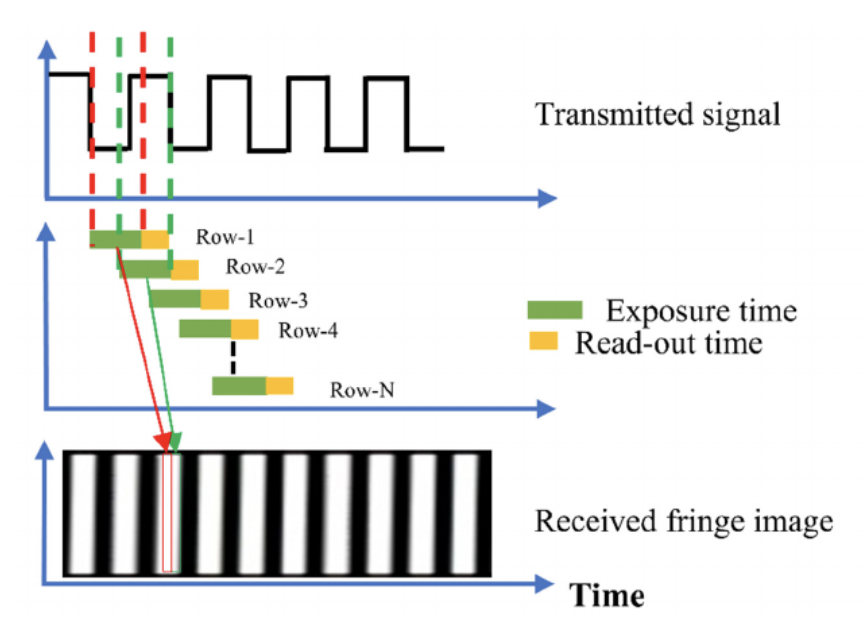
\includegraphics[width=8cm]{ch2pic/rolling_shutter.png}
                        \caption{滾動式快門效應的成因\cite{pic:rolling_shutter}}
                        \label{pic:rolling_shutter}
                    \end{figure}

                    \begin{figure}[ht]
                        \centering
                        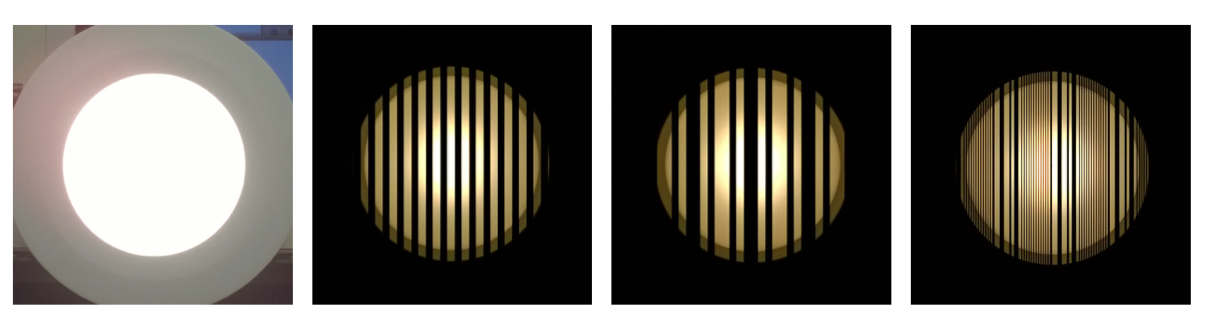
\includegraphics[width=8cm]{ch2pic/rolling_shutter_case.png}
                        \caption{滾動式快門效應產生的條紋樣式\cite{pic:rolling_shutter_case}}
                        \label{pic:rolling_shutter_case}
                    \end{figure}

                    \qquad
                    光波段中除了環境光源會造成誤差以外,誤差主要來源於多重路徑傳輸,如圖\ref{pic:multipath}所示,訊號在傳送至感測器之前,由於障礙物造成訊號反射,使得感測器接收的訊號除了LoS路徑以外,還包含了透過反射傳送而來的訊號。除了LoS訊號以外,感測器量測到的NLoS訊號,便會造成誤差。而相機使用的為影像中的特徵點,因此較不受多重路徑傳輸的影響,在此相誤差上具有優勢。

                    \begin{figure}[ht]
                        \centering
                        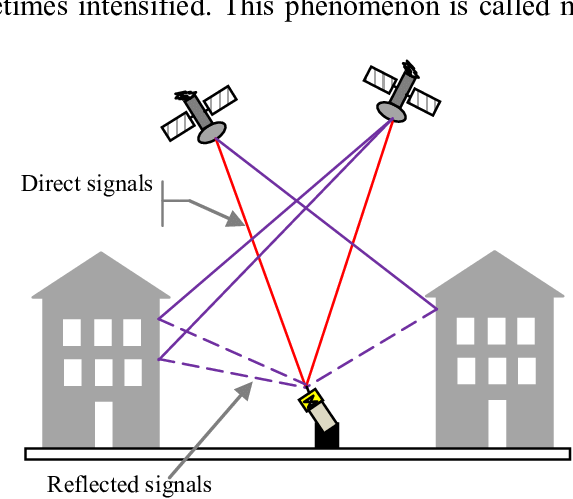
\includegraphics[width=6cm]{ch2pic/multipath.png}
                        \caption{多重路徑傳輸\cite{pic:multipath}}
                        \label{pic:multipath}
                    \end{figure}

                    \item[- PD]\hfill
                    
                    \qquad
                    PD能感測到資訊僅有強度資訊,而強度資訊受LED出射角度、PD入射角度、距離影響(詳細參考\ref{chp:LEDPD_radiate}章),相較大多無線電波技術主要僅受距離影響,PD的變數較多,使得獲得相對定位的演算法較複雜,也需要多個PD或多個LED以進行定位。然而PD優勢為具有極高的取樣頻率,可高達千赫茲甚至萬赫茲,高取樣頻率即可使用光通訊進行編碼與解碼,且硬體成本相較影像感測器來說非常低。

                    \qquad
                    PD定位系統的架構如圖\ref{pic:vlc_flow}所示,訊號發送是利用驅動器與LED進行光通訊,PD接收訊號後進行解碼、取得LED的ID與與光強度,再利用光強度以不同演算法解出相對位置。而LED與PD的定位系統中,包含單LED對多PD、多LED對多PD、或是多LED對多PD,其中,當系統內包含多個LED對多PD時,PD會同時接收到來自多個LED的編碼訊號,參考圖\ref{pic:vlc_multi_pd},PD會將訊號轉換至頻域,以獲得各頻率下的強度,也就是各LED傳送至各PD的強度。

    
                    
                    \begin{figure}[ht]
                        \centering
                        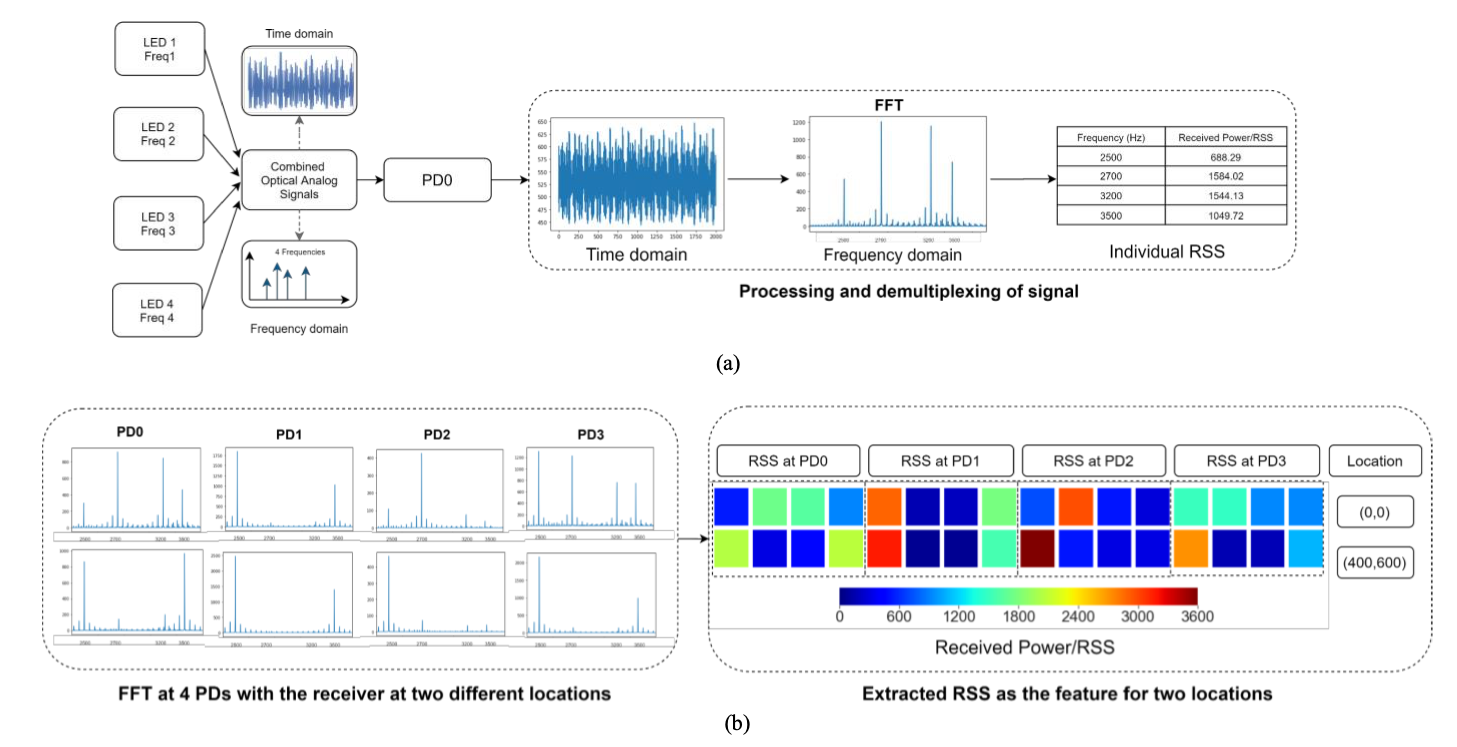
\includegraphics[width=15cm]{ch2pic/vlc_multi_pd.png}
                        \caption{多PD進行光通訊解碼\cite{case:ml}}
                        \label{pic:vlc_multi_pd}
                    \end{figure}

                    \qquad
                    利用光通訊獲得各LED傳送至各PD的強度後,解出定位的演算法分成兩類,一類型為使用指紋法或多點定位,這種類型的系統需在環境中放置多個參考點(如圖\ref{pic:env_finger}),為「環境對一點的定位」。除此之外,大多使用\ref{chp:method-algorithm}章中提到的幾何方法,如\cite{case:3d_layers}(參考圖\ref{pic:env_1to1}),透過多PD量測強度後,利用多個PD強度與幾何之間的關係取得定位,此類型方法詳述於\ref{chp:LEDPD_problem}章。

                    \begin{figure}[ht]
                        \centering
                        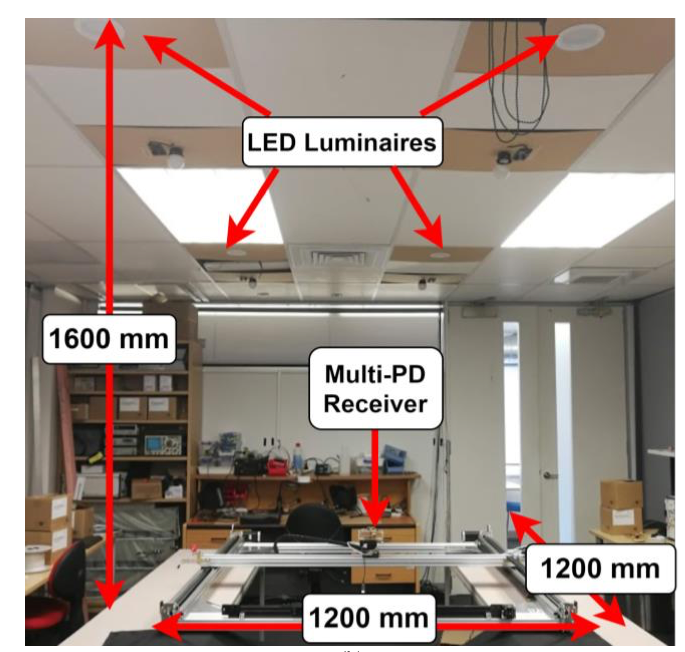
\includegraphics[width=8cm]{ch2pic/env_finger.png}
                        \caption{使用指紋法的系統環境\cite{case:ml}}
                        \label{pic:env_finger}
                    \end{figure}

                    \begin{figure}[ht]
                        \centering
                        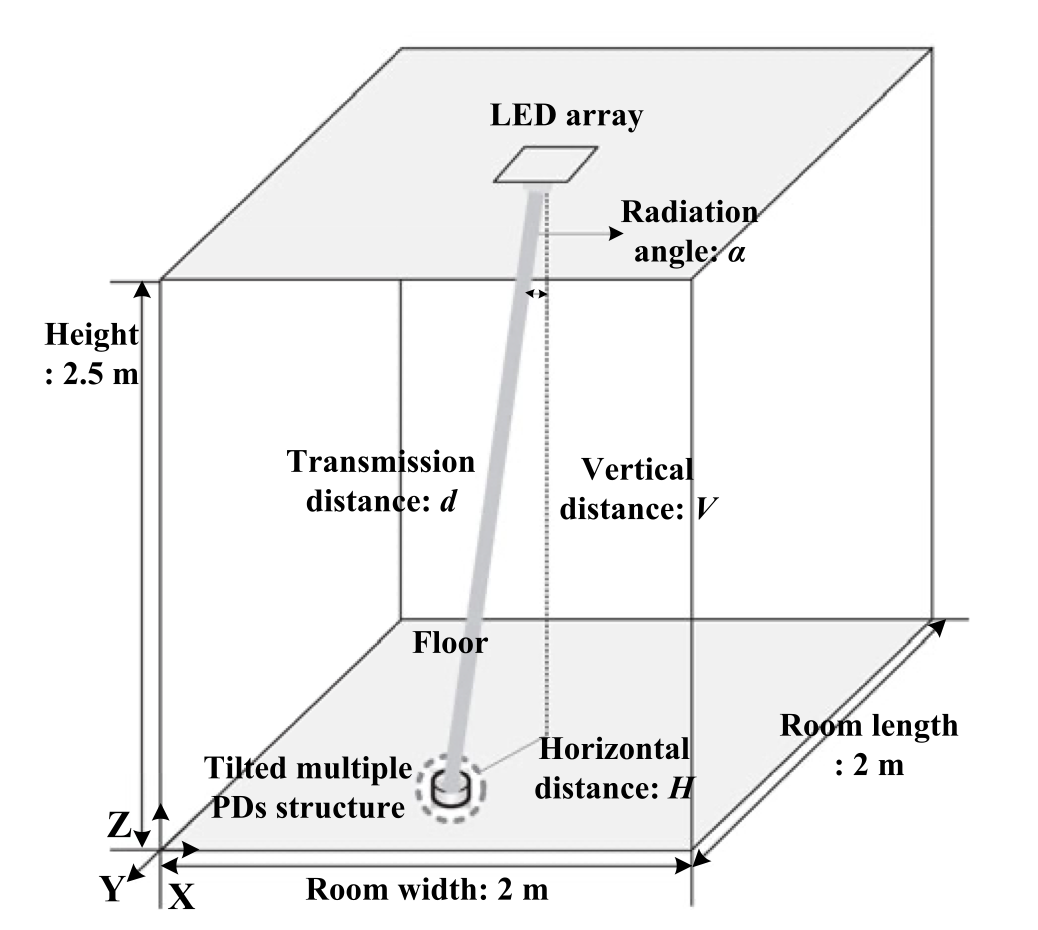
\includegraphics[width=8cm]{ch2pic/env_1to1.png}
                        \caption{使用幾何方法的系統環境\cite{case:3d_layers}}
                        \label{pic:env_1to1}
                    \end{figure}

                \end{description}

                影像感測器與PD進行定位的方法差異非常大,前者演算法為影像辨識,利用特殊圖案分辨光源,以影像中的變形計算位置;PD常見的定位演算法則包含多點定位、指紋法、幾何方法,利用光通訊分辨光源。在兩者之間權衡時,本研究主要考量到成本以及硬體大小,為了能夠達到靈活、廣泛運用,取捨掉影像感測器具有高精度可能性的優勢。


                \begin{figure}[ht]
                    \centering
                    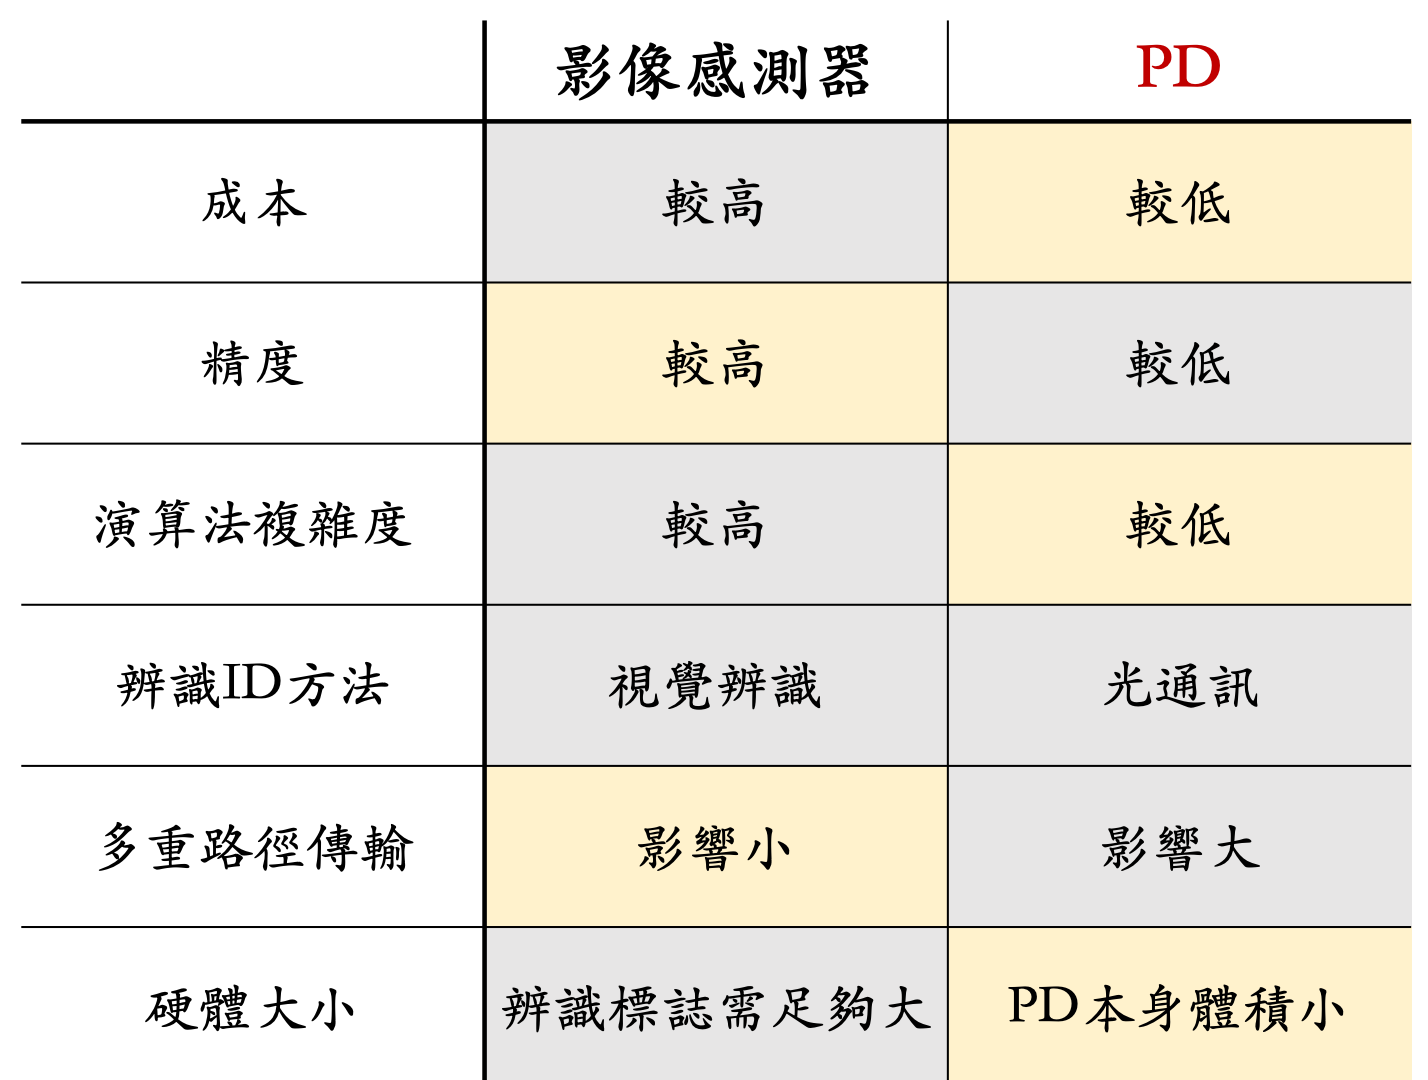
\includegraphics[width=9cm]{ch2pic/pd_camera_sort.png}
                    \caption{影像感測器與PD的特性比較}
                    \label{pic:pd_camera_sort}
                \end{figure}

                


        
                

        \subsection{小結:本研究使用技術的選擇}
        

        在\ref{chp:technique}章中,由電磁波頻率分類為無線電波段與光波段,分別於\ref{chp:radio}章與\ref{chp:light}章中介紹無線電波與光波段的定位,並於\ref{pic:method_compare}中比較兩者,其中光波段較高的精度、較小的硬體、以及能夠零或應用的幾何方法演算法,使光波段定位為更適合的選擇。

        光波段中,又依照使用波段與使用的硬體分類。使用波段於\ref{chp:light_electro}章中討論,分為可見光、近紅外光與遠紅外光,參考圖\ref{pic:light_freq_compare},近紅外光兼具低成本低干擾的特色,因此選用近紅外光波段中,位於輻射光譜低谷的760nm與940nm波段最為合適。硬體選擇則於\ref{chp:light_receiver}章中討論,參考圖\ref{pic:pd_camera_sort},權衡之下選擇PD,雖然捨棄精度,但得以換取較低的成本與較小的體積;另外,PD所使用的定位演算法需為具有靈活度的幾何方法。
    
        
        綜上所述,本論文將使用LED與PD的定位方法,於後續的\ref{chp:LEDandPD}章中更深入的討論,分別介紹LED與PD的特性、光傳遞模型,以及現今文獻所遇困難與限制。


        

    

        

        

        

        


        

        

            

          

        


\section{LED與PD的定位方法}
\label{chp:LEDandPD}
    


    
    於\ref{chp:technique}章中,我們將定位方法聚焦在LED與PD的定位方法上,而此種系統是將單個或多個LED安裝在目標物上,各LED藉由編碼來區別各自的訊號,而PD安裝於觀察物上,將每個PD所接收的訊號分別解碼,得到各LED的訊號強度。

    為深入了解系統運作方式,從\ref{chp:light_unit}章開始介紹常用的光學單位;有基本了解後,於\ref{chp:LEDPD_radiate}介紹LED與PD的輻射特性。了解輻射特性後,於\ref{chp:model}中介紹完整的光傳遞模型,最後再進入\ref{chp:LEDPD_problem}介紹現今文獻的作法,並整理所遇困難與限制。



    \subsection{光學常用單位介紹}
    \label{chp:light_unit}
        
        由於光領域所使用的單位與機械領域差距較大,且單位與術語經常有口語或混用的情況,令人感到困惑,因此在進入PD與LED定位的探討之前,先對光領域的一些術語與單位進行介紹。

        首先,描述光照的單位分為兩種系統,輻射測量學(Radiometry)與光度測量學(Photometry),兩領域以不同單位描述光源,其中輻射測量學著重在電磁波輻射的量測,描述通量單位為瓦特(Watt);而光度測量學著重在人演可見之可見光波段的研究,通量單位為流明(Lumen),同樣物理量下單位定義不同\cite{radiometry_and_photometry}。
        

        \begin{figure}[ht]
            \centering
            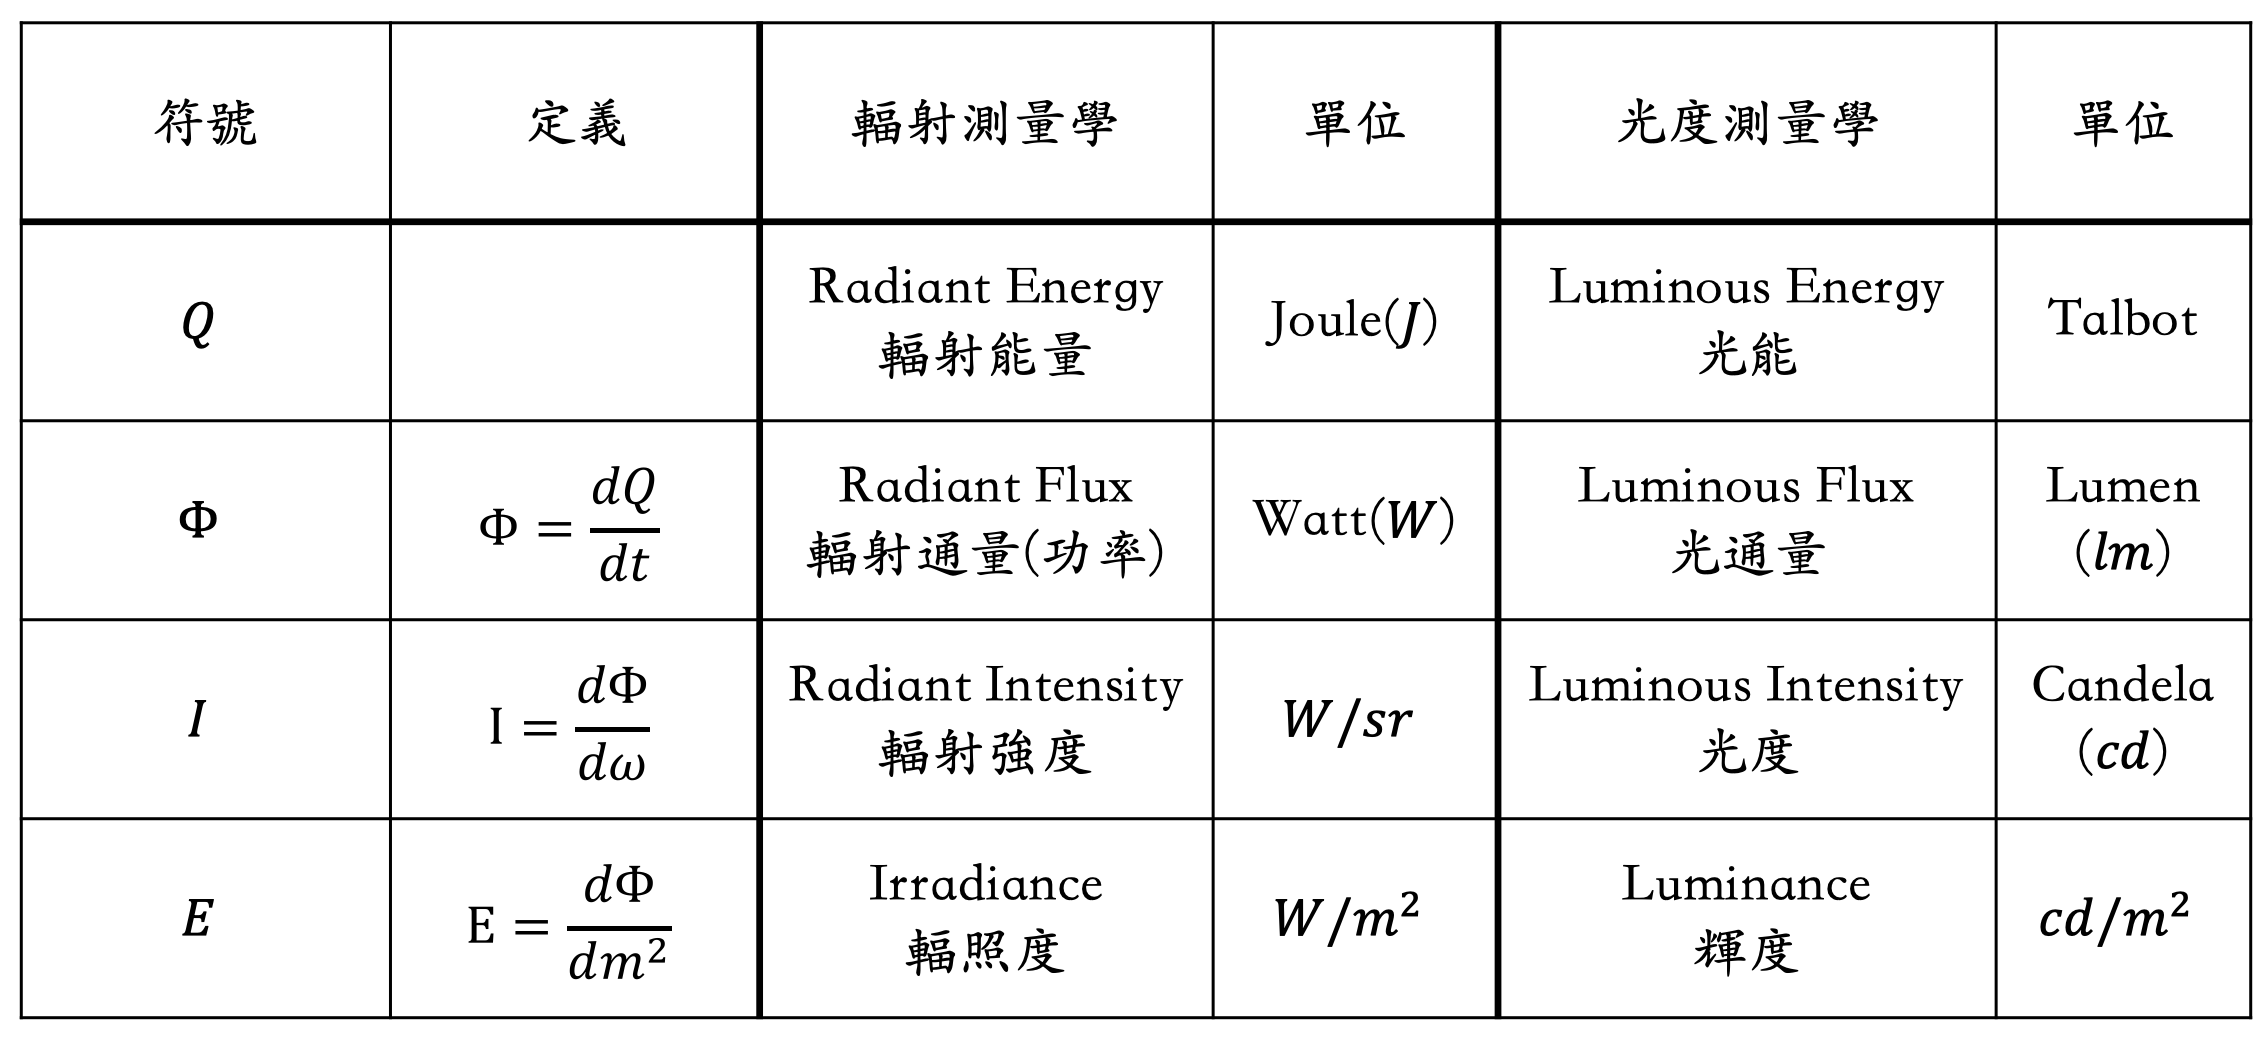
\includegraphics[width=14cm]{ch2pic/photometry_table.png}
            \caption{輻射測量學與光度測量學的物理量比較}
            \label{tab:photometry}
        \end{figure}


        本研究聚焦在近紅外光波段,因此本論文會使用輻射測量學的系統,然而文獻上可見光定位數量較多,因此在單位的換算上需特別注意,以下針對光領域常用物理量分項簡單介紹。

        
        \begin{description}
            \item[- 立體角 Solid Angle $\Omega$] \hfill
                
                \qquad
                描述二維空間中的角度單位為弧度,代表夾角內的弧長與半徑比例,而單位弧度的定義是半徑與圓弧長度相等時的圓心角。
                \qquad
                然而光源存在於立體空間中,而空間中描述角度的物理量即為立體角$\Omega$(Solid Angle),該物理量代表一光束投影於單位球面上時,表面積與半徑平方的比例,如圖\ref{pic:solid_angle}所示。立體角的單位為球面度(steradians, 簡寫$sr$)代表在半徑為$r$的球體中,立體角投射出的表面積為$r^2$。

                \begin{figure}[ht]
                    \centering
                    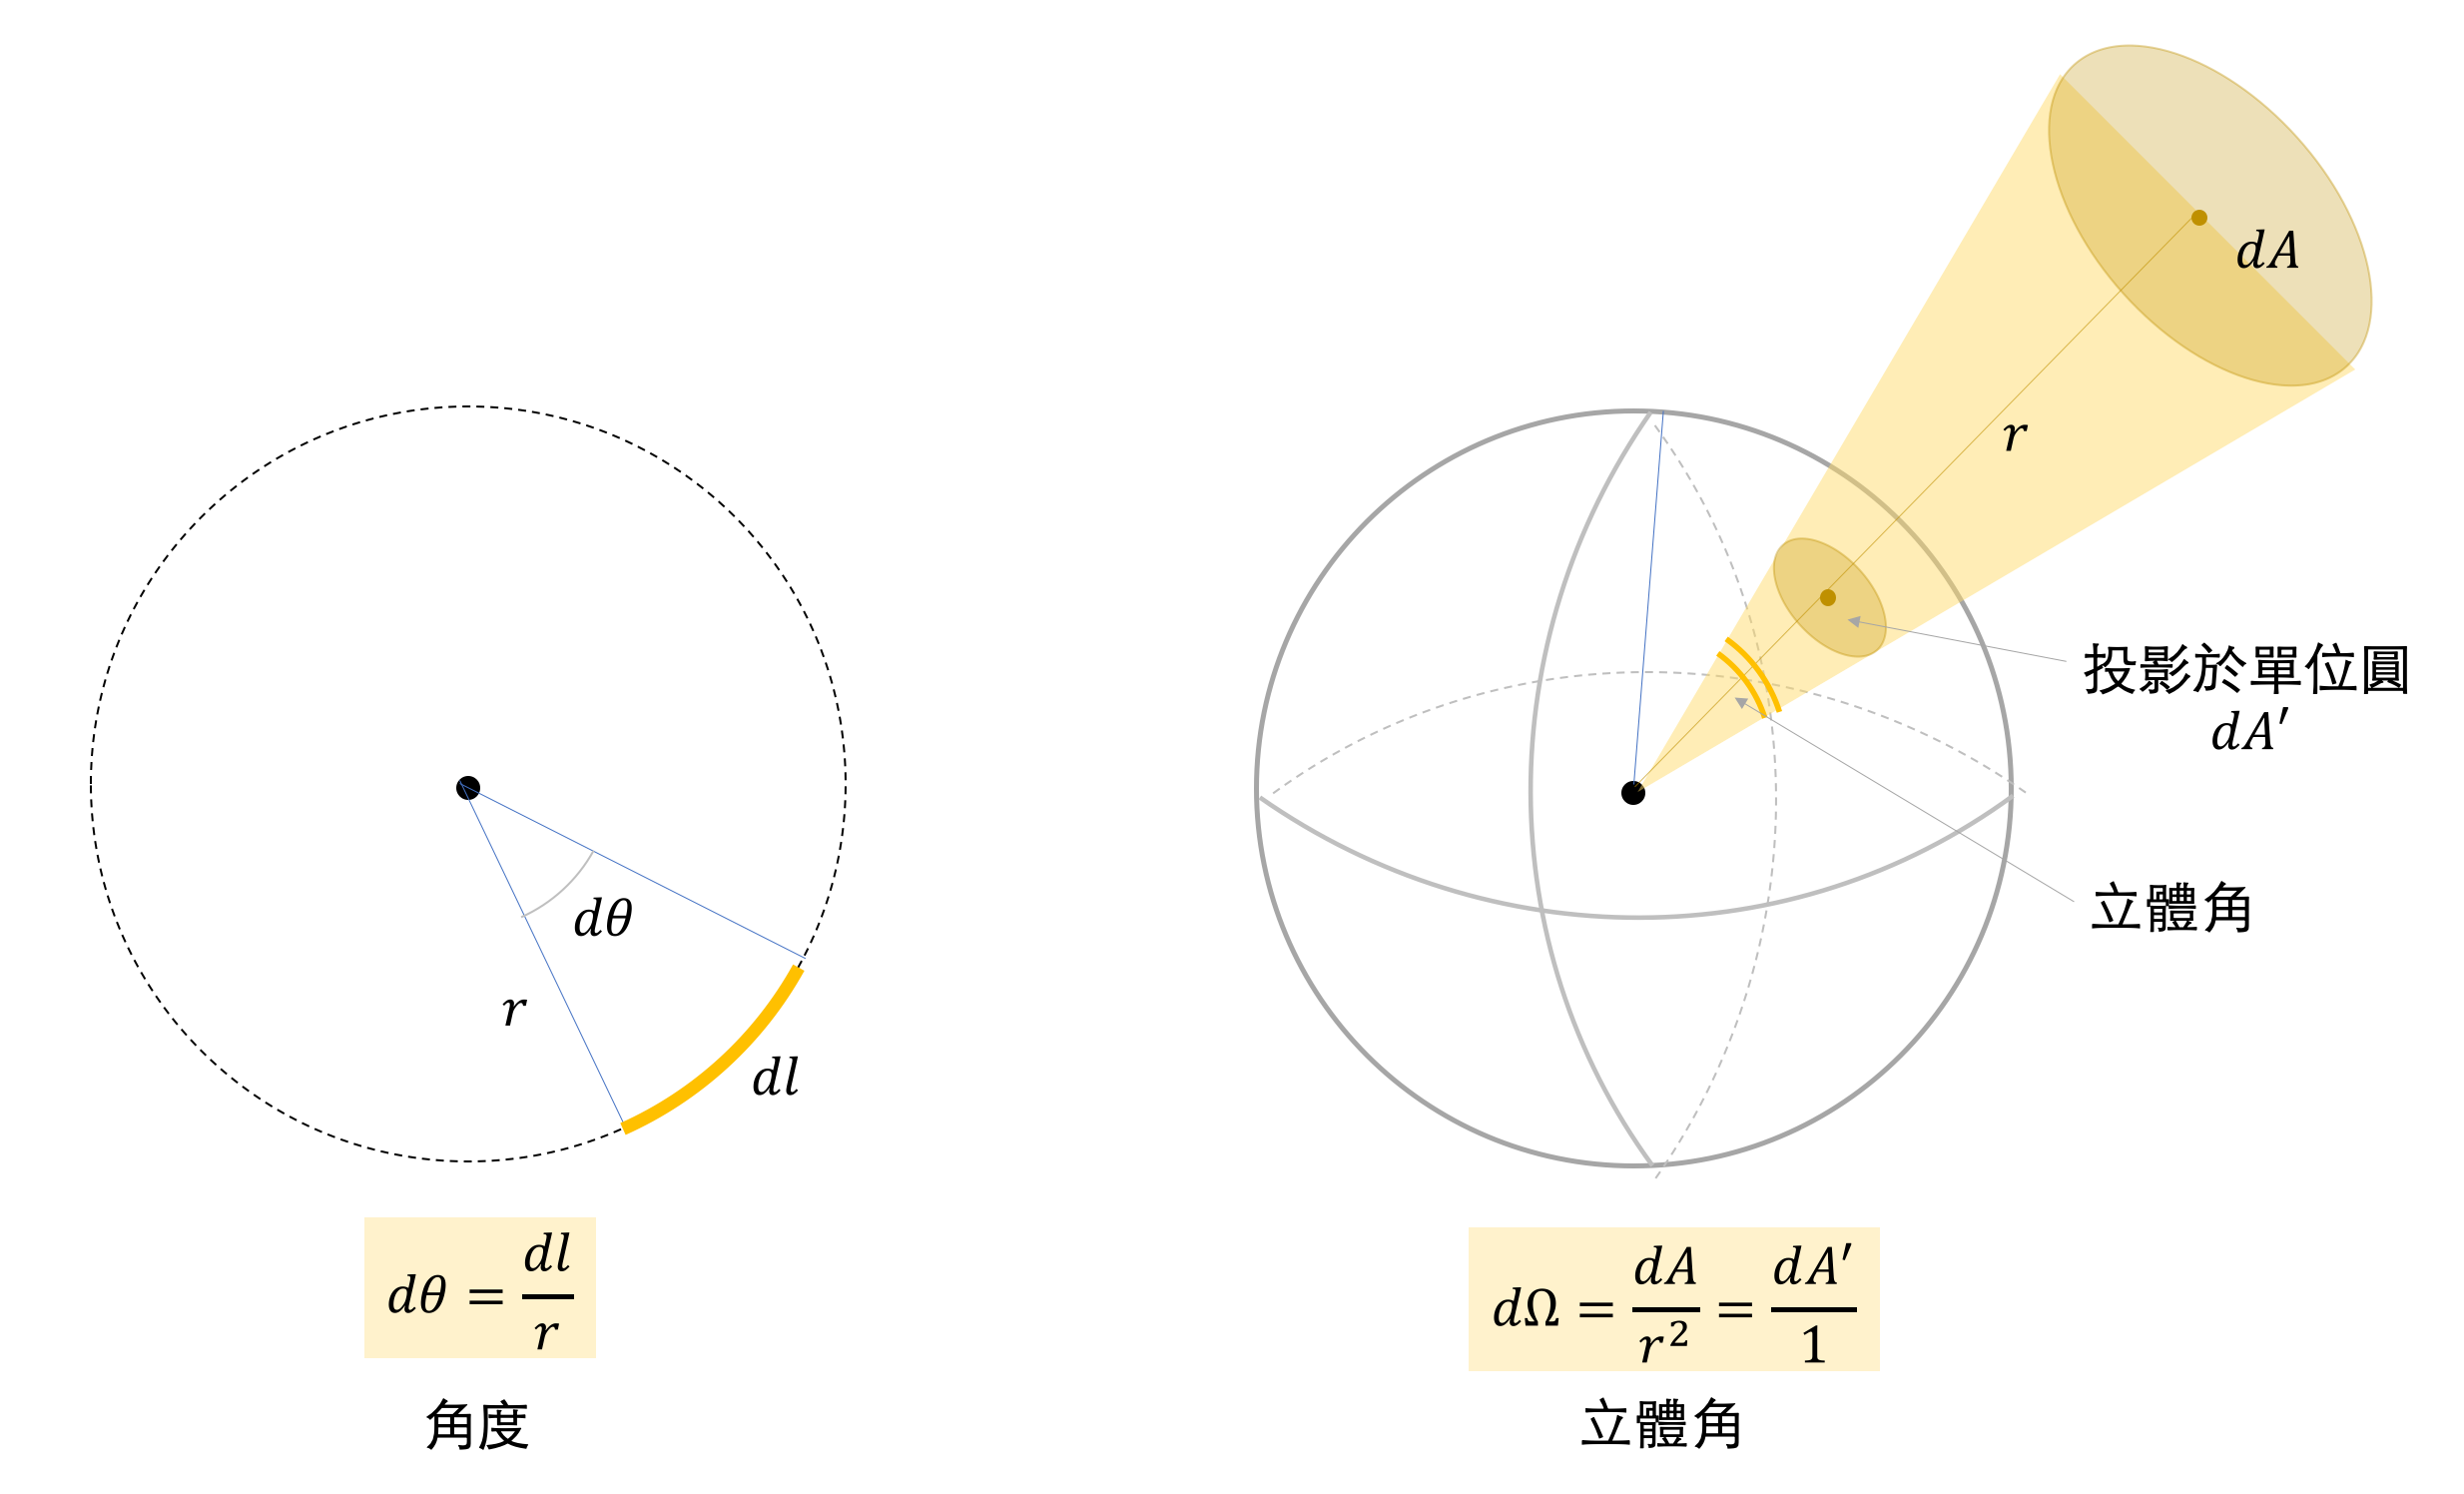
\includegraphics[width=12cm]{ch2pic/solid_angle.png}
                    \caption{角度與立體角}
                    \label{pic:solid_angle}
                \end{figure}

            \item[- 輻射通量 Radiant Flux $\Phi$]  \hfill
                
                \qquad
                描述光照功率的物理量為通量(Flux)或稱輻射功率(Power),用符號$\Phi$表示,代表每單位時間的輻射能量,單位為瓦特,而大多LED規格表上以此物理量來描述LED在指定電流下可產生的最大光功率。

            \item[- 輻射強度 Radiation Intensity $I$] \hfill
             
                \qquad
                每單位立體角所含的通量稱為輻射強度$I$,此物理量常用於描述光與立體角之關係,在同一光束內,輻射強度僅與立體角有關,與距離無關。

                \begin{figure}[ht]
                    \centering
                    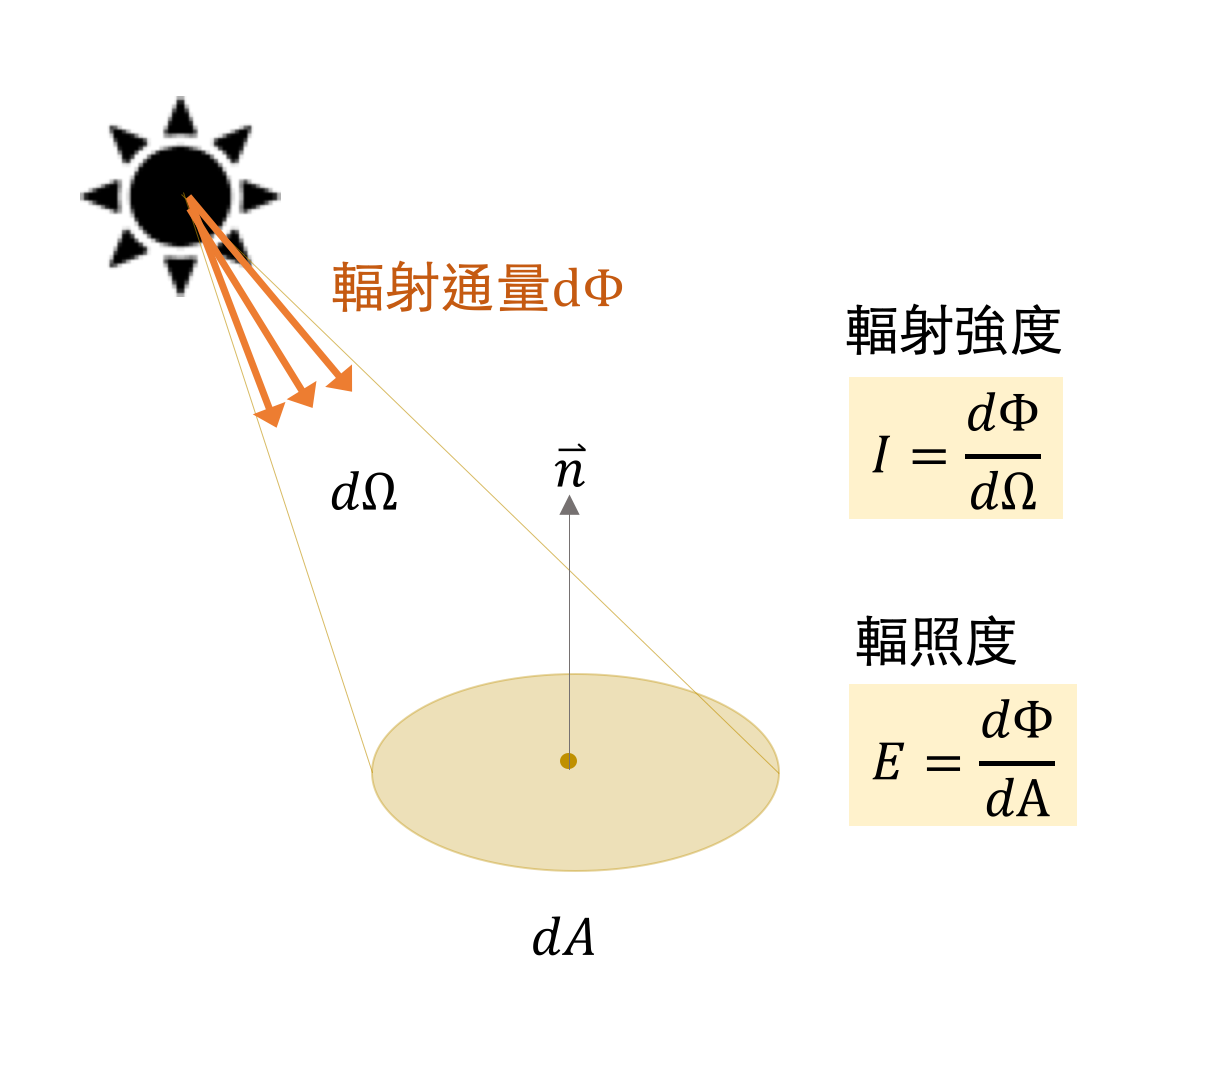
\includegraphics[width=8cm]{ch2pic/intensity_irradiance.png}
                    \caption{輻射強度與輻照度}
                    \label{pic:intensity_irradiance}
                \end{figure}

            \item[- 輻照度 Irradiance $E$] \hfill
                
                \qquad
                每單位面積所含的通量稱為輻照度(參考圖\ref{pic:intensity_irradiance}),其中照射面積隨著距離$D$增加而平方遞增。

                
                % \begin{equation}
                %     \label{eqn:I2E}
                %     E=I\cos\omega/D^2
                % \end{equation}      
             
        \end{description}

        

        

    \subsection{LED與PD的輻射特性}
    \label{chp:LEDPD_radiate}

    LED與PD硬體有許多種類,最常見的市面上LED與PD為軸對稱並滿足朗博輻射模式(Lambertian Radiation Pattern),本論文僅考慮此類硬體,其中軸對稱代表輻射強度並不隨方位角改變。

    以下章節依序從\ref{chp:lambertian}章起,介紹LED與PD皆遵守的朗博輻射模型(Lambertian Radiation Pattern),再於\ref{chp:LED}與\ref{chp:PD}分別介紹LED與PD兩者各自的硬體特性。
    
        
        \subsubsection{朗博輻射模型}
        \label{chp:lambertian}

        

        LED與PD的照射與接收模式(Pattern)皆可以用朗博輻射模式描述(圖\ref{pic:lambertian}),其代表感(發)光強度隨著LED出射角(PD入射角)的增加而衰減,如式\ref{eqn:lambertian_pattern}其衰減模式可用餘弦函數(cosine)的$M$次方(power)表示,$M$代表的是朗博次方(Lambertian Order)。

        \begin{equation}
            \label{eqn:lambertian_pattern}
            I(\omega)=I(\omega=0)\times\cos(\omega)^{M}\\
        \end{equation}

        \begin{figure}[ht]
            \centering
            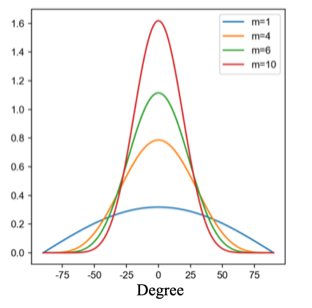
\includegraphics[width=8cm]{ch2pic/lambertian.png}
            \caption{輻射強度與出入射角的關係}
            \label{pic:lambertian}
        \end{figure}

        以二維的角度來看如圖\ref{pic:lambertian},LED光照射的能量隨出射角度增加而減少,在LED中心軸的方向有最高的輻射強度,需注意的是輻射強度與距離無關(參考\ref{chp:light_unit}章)。如先前所述,LED為軸對稱,因此三維的照射模式即為二維模式以中心軸旋轉,參考圖\ref{pic:lambertian_3d},在同樣出射角下,光輻射強度相同。
        
        \begin{figure}[ht]
            \centering
            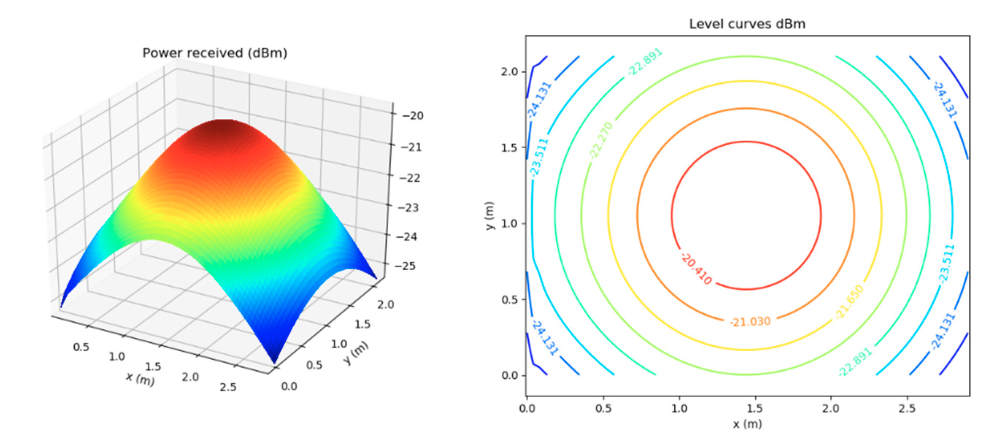
\includegraphics[width=12cm]{ch2pic/lambertian_3d.png}
            \caption{輻射強度與出入射角的關係}
            \label{pic:lambertian_3d}
        \end{figure}

        朗博次方所代表的意義,可視為在敏感度與照射範圍中的取捨:朗博次方較小時,其照射範圍較大,最大可以覆蓋接近半個球面,光強度隨出射角度衰減的速度不大,也就是對不同入射角度的敏感度則不高。反之,朗博次方較大的硬體雖然覆蓋範圍較小,但對覆蓋範圍內的角度變化敏感度高(如圖\ref{pic:lambertian})。

        

        \subsubsection{LED特性}
        \label{chp:LED}

        LED與PD在選購時,除了挑選朗博次方以外,也需注意其他特性以及影響發收光能力的硬體參數,在此將硬體參數整理於圖\ref{pic:hardware_para},這些硬體參數會陸續於\ref{chp:LED}與\ref{chp:PD}中介紹。
        
        \begin{figure}[ht]
            \centering
            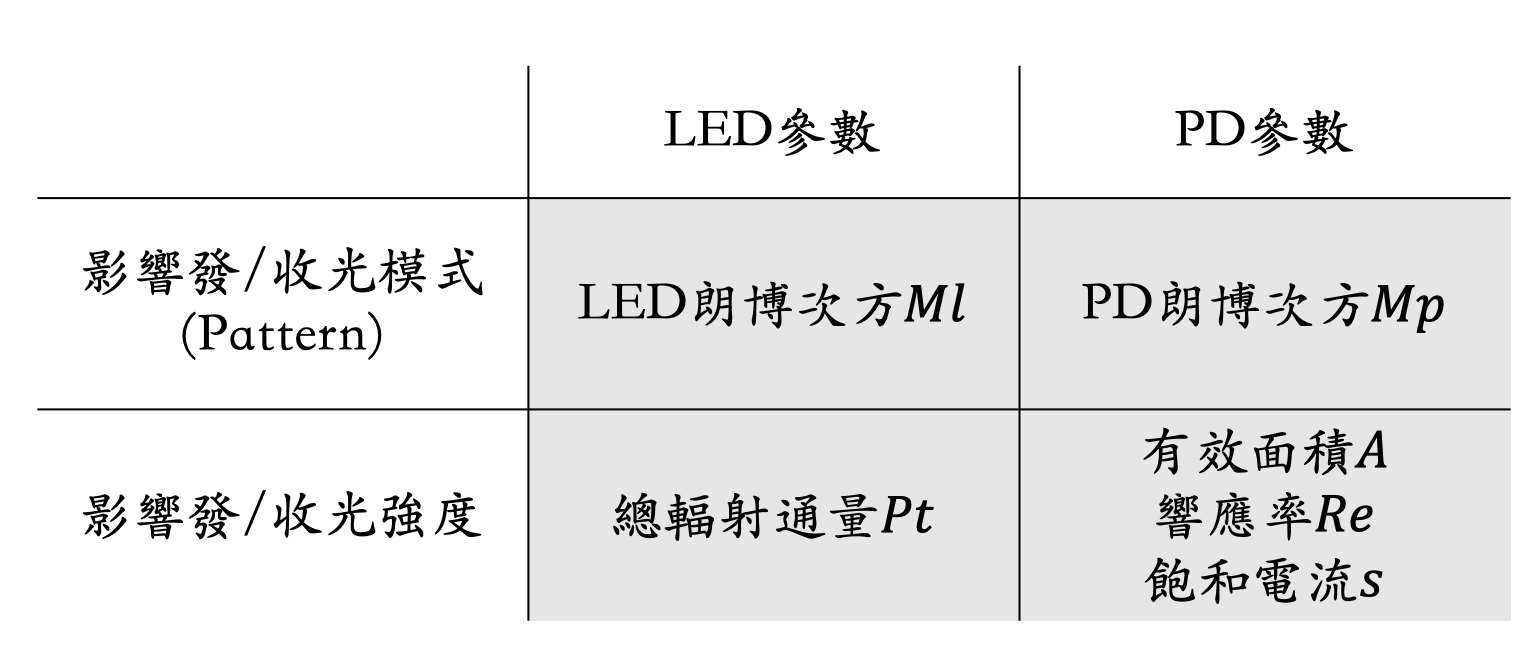
\includegraphics[width=9cm]{ch2pic/hardware_para.png}
            \caption{LED與PD的硬體參數}
            \label{pic:hardware_para}
        \end{figure}

        LED發出的輻射,會遵守式\ref{eqn:lambertian_pattern}描述的朗博輻射模式,其提供了光輻射強度$I$與不同出入射角$\omega$的關係,在此部分僅討論LED,因此變數為出射角$\theta$,而LED的輻射強度以$Il$表示。由於光輻射為軸對稱照射於空間中,因此需將整個半球中的輻射強度積分,得到$Pt = Il(0)(Ml+1)/2\pi$,移項即可完成式\ref{eqn:lambertian_led}。此式描述LED輻射強度$Il$與入射角度、LED總輻射功率以及朗博次方的關係。
        
    
        \begin{equation}
            \label{eqn:lambertian_led}
            Il(\phi)=Pt\frac{(Ml+1)}{2 \pi} \cos \theta^{Ml}
        \end{equation}





        \subsubsection{PD特性}
        \label{chp:PD}

        首先,PD得到的輻射強度$Ip$也遵守朗博輻射模式,\ref{eqn:pd_I}描述輻射強度與入射角度$\phi$以及PD朗博次方$Mp$的關係。

        \begin{equation}
            \label{eqn:pd_I}
            Ip(\phi) = Il \cos \phi^{Mp}
        \end{equation}

        而PD所量測到的為輻射通量$\Phi$,再將輻射通量轉換為電流輸出(式\ref{eqn:pd_current})。而輻射通量可藉由圖\ref{pic:intensity_irradiance}中輻射通量與輻射強度的關係,以及立體角$\Omega$的定義換算,於式\ref{eqn:pd_flux}將式\ref{eqn:pd_I}的光強度轉換為PD接收的輻射通量。其中,$A$為PD的硬體參有效面積,$D$為LED與PD之間的距離。

        \begin{equation}
            \label{eqn:pd_flux}
            \Phi p = \frac{Ip}{\Omega} = \frac{IpA}{D^2}
        \end{equation}

        而PD最終輸出電流$Ie$與輻射通量$\Phi p$的關係由式\ref{eqn:pd_current}描述,$s$為PD的飽和電流,也就是該PD能夠輸出的最大電流。

        \begin{equation}
            \label{eqn:pd_current}
            Ie = \begin{cases}\Phi\times Re, & \text { if } Ie<s \\ s, & \text { otherwise }\end{cases}
        \end{equation}

        綜合式\ref{eqn:pd_I}、式\ref{eqn:pd_flux}、式\ref{eqn:pd_current},PD輸出的電流$Ie$與LED的輻射強度$Il$統整於式\ref{eqn:pd},式中的硬體參數可參考圖\ref{pic:hardware_para}:

        \begin{equation}
            \label{eqn:pd}
            Ie = \begin{cases}Re \frac{A}{D^2}Il(\theta) \cos \phi^{Mp}, & \text { if } Ie<s \\ s, & \text { otherwise }\end{cases}
        \end{equation}

        
        


        

    \subsection{光傳遞模型}
    \label{chp:model}

    本章節將綜合\ref{chp:LED}章與\ref{chp:PD}章中呈現的LED與PD模型,於\ref{chp:model_1to1}章中,呈現由LED光源將光波傳送至PD並轉換成電流的模型;皆著於\ref{chp:model_mul}章中,將LED與PD的數量提升為多個;最後於\ref{chp:model_transform}中將距離、出入射角變數轉換為用相對位置表示,呈現出LED與PD在不限制條件的情況下,模型的複雜度。
    
    \subsubsection{單LED對單PD光傳遞模型}
    \label{chp:model_1to1}

    光傳遞模型需建立由LED至PD的過程,LED與PD各自的輻射與接收特性分別於\ref{chp:LED}章與\ref{chp:PD}章中介紹,綜合描述LED發光強度$Il$的式\ref{eqn:lambertian_led},以及描述PD輸出電流$Ie$的式\ref{eqn:pd},即可獲得一LED對一PD的光傳遞模型(式\ref{eqn:model_1to1})。

    \begin{equation}
        \label{eqn:model_1to1}
        Ie = \begin{cases}Re \cdot A\cdot Pt\frac{Ml+1}{2\pi}\frac{\cos \phi^{Mp}\cos \theta^{Ml}}{D^2}, & \text { if } Ie<s \\ s, & \text { otherwise }\end{cases}
    \end{equation}

    在光傳遞模型中,與定位相關的變數包含三個:距離$D$、PD入射角$\phi$、LED出射角$\theta$,他們便是幾何方法演算法要使用的變數。其中出入射角如圖\ref{pic:interactive_1to1},分別為硬體中心軸與距離向量之間的夾角。

    \begin{figure}[ht]
        \centering
        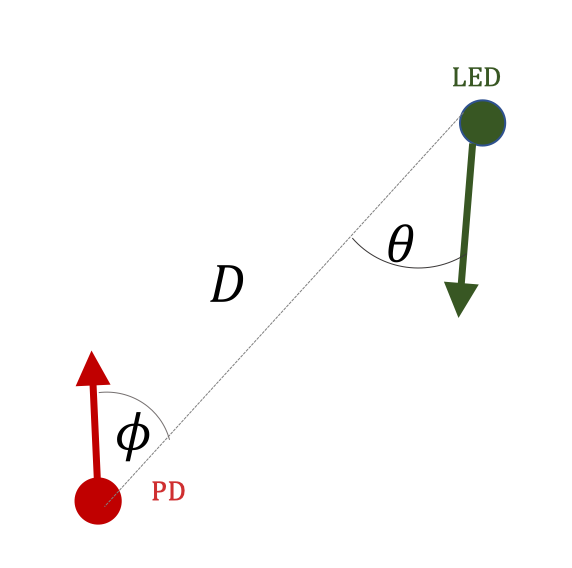
\includegraphics[width=6cm]{ch2pic/interactive_1to1.png}
        \caption{單LED與單PD的交互關係}
        \label{pic:interactive_1to1}
    \end{figure}

    \subsubsection{多LED對多PD光傳遞模型}
    \label{chp:model_mul}

    由於LED與PD定位時數量通常不只一個,因此描述多LED對多PD的光傳遞模型時,需註明清楚(可參考\ref{chp:symbol})。在此設定LED總數為$L$、PD總數為$P$,描述第$l$個LED與第$p$個PD的硬體參數時,於硬體參數的右下標加註,如$A_2$為第二個PD的有效面積;再來,描述第$l$個LED與第$p$個PD之間的關係時,則將$lp$同樣加註於右下標,例如$D_34$為第三個LED與第四個PD之間的距離,參考圖\ref{pic:interactive_mul}。
    
    \begin{figure}[ht]
        \centering
        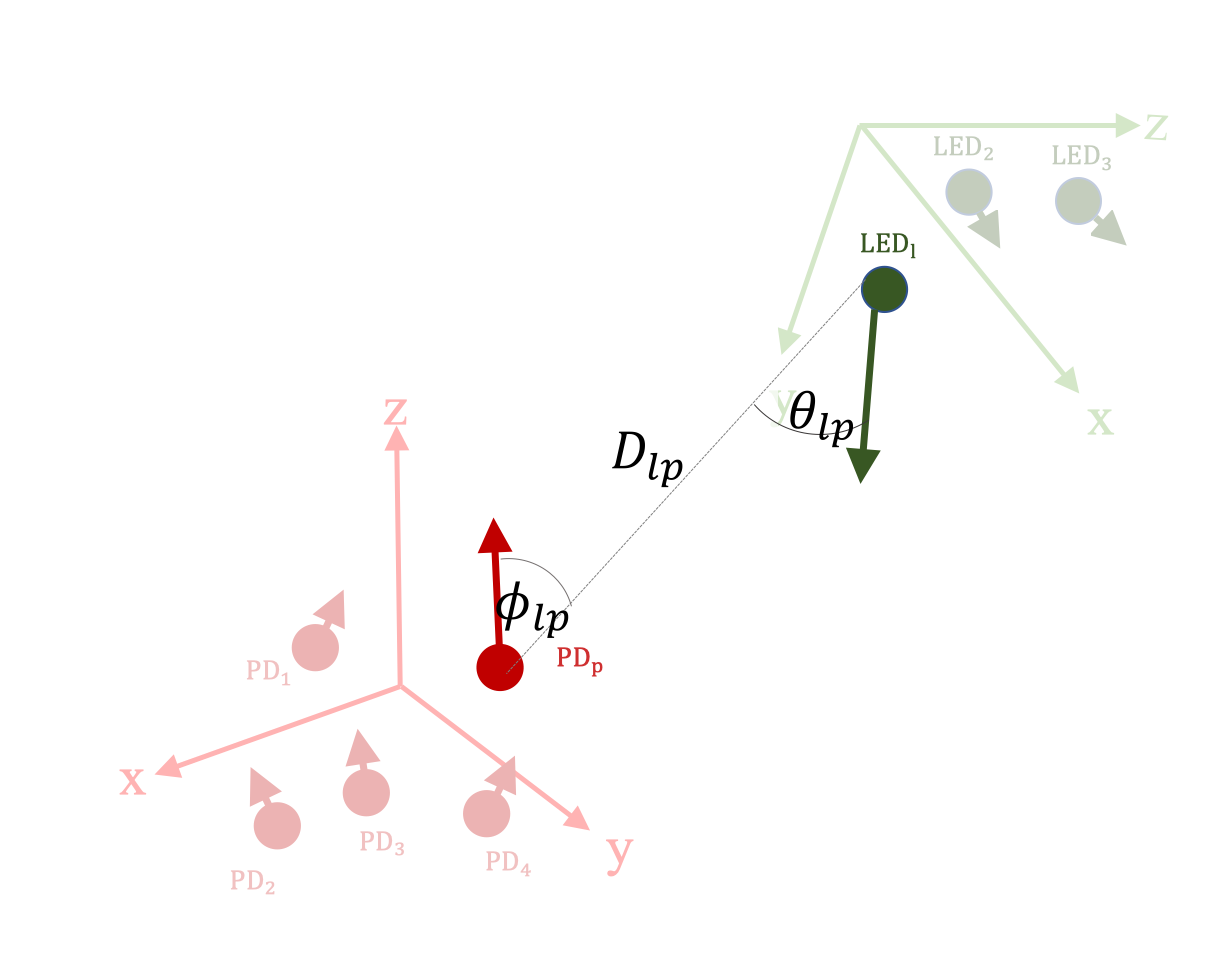
\includegraphics[width=8cm]{ch2pic/interactive_mul.png}
        \caption{多LED與多PD的交互關係}
        \label{pic:interactive_mul}
    \end{figure}

    而完整的多LED對多PD的的模型如式\ref{eqn:model}
    
    \begin{equation}
        \label{eqn:model}
        Ie = \begin{cases}Re \frac{ A_p\cos\phi_{lp}^{Mp_{p}} }{D^2_{lp}}\times Pt_l\frac{(Ml_{l}+1)}{2 \pi} \cos \theta_{lp}^{Ml_{l}}, & \text { if } Ie<s \\ s, & \text { otherwise }\end{cases}
    \end{equation}




    \subsubsection{統整光傳遞模型與座標轉換}
    \label{chp:model_transform}

    在\ref{chp:relative}章中,我們以兩個座標系表示LED與PD各自為剛體,也定義了兩座標系之間的齊次座標轉換矩陣為$^{PL}\boldsymbol{H}$,左上標的$PL$代表將LED座標系投影至PD座標系上。在目標情境中,LED與PD座標系各自可移動、旋轉,而LED與PD各自固定於自己的座標系,而目標得到的位置資訊即為平移矩陣$^{PL}\boldsymbol{T}$。

    我們要使用幾何方法類型的演算法,因此需利用光傳遞模型中(式\ref{eqn:model}),輸出電流與距離、出入射角間的關係,計算出平移矩陣$^{PL}\boldsymbol{T}$。因此我們需利用座標轉換,將LED座標系上的LED擺設,轉換至PD座標系上,以進行距離、出入射角的計算。

    圖\ref{pic:model_transform_flow}為將光傳遞模型與相對定位統整的流程,首先我們需定義LED與PD各自在座標系上的擺放自由度;定義好各自固定於座標系上的位置後,透過齊次座標轉換,將LED投影到PD座標系上;最後於PD座標系上計算各LED與PD的距離、出入射角。

    \begin{figure}[ht]
        \centering
        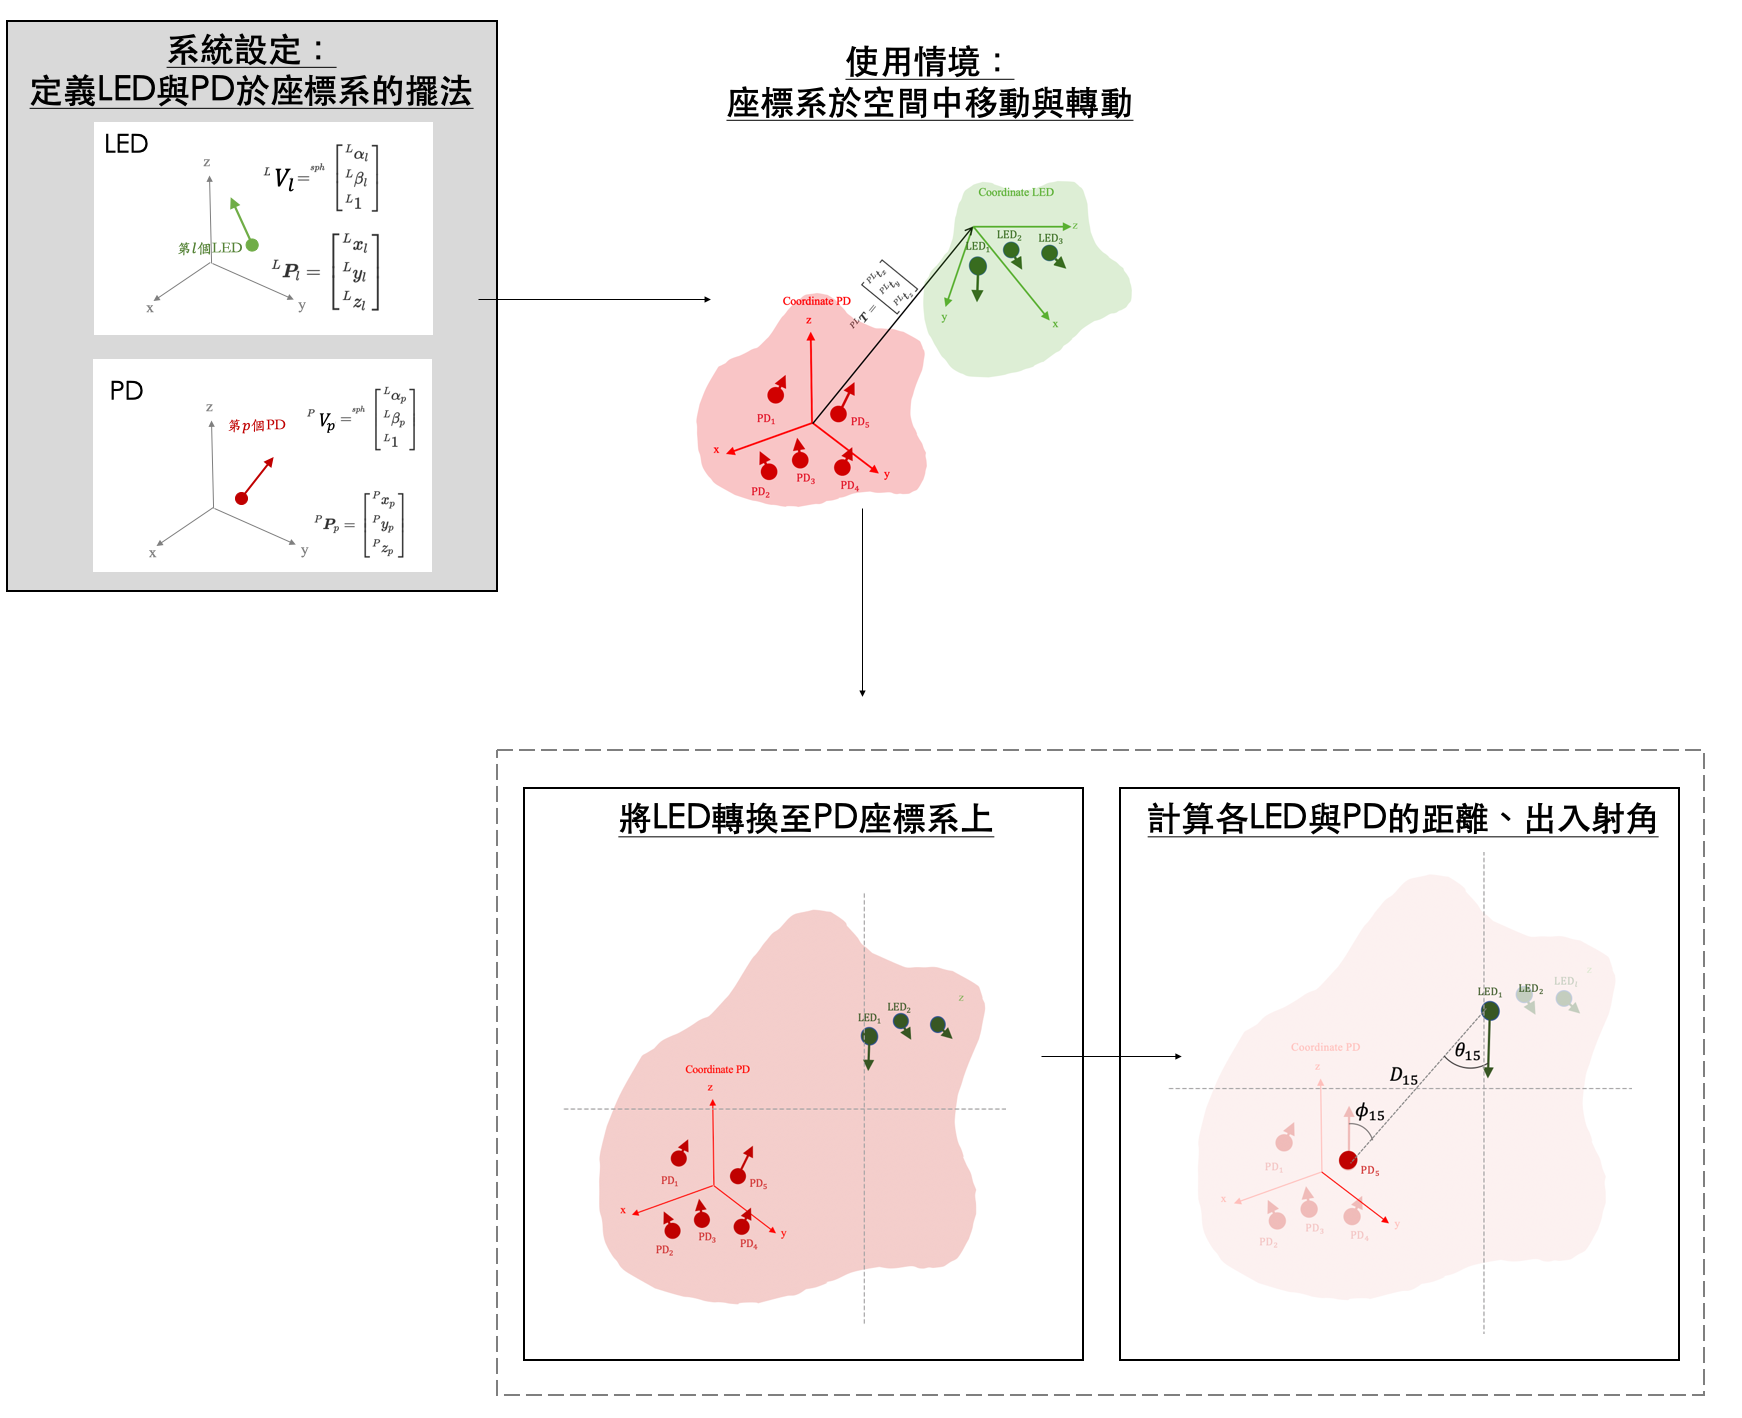
\includegraphics[width=15cm]{ch2pic/model_transform_flow.png}
        \caption{光傳遞模型與相對定位統整的流程}
        \label{pic:model_transform_flow}
    \end{figure}
    
    \begin{description}

        \item[- 定義LED與PD於各自座標系上的擺法]\hfill 
        
        \qquad
        在描述座標系空間中的LED與PD時,一共有五個自由度,包含擺放位置$P$的三個分量$x,y,z$,以及定義指向的單位向量$V$。由於LED與PD皆為軸對稱,因此僅有兩個自由度:天頂角$\alpha$與方位角$\beta$,$V$在卡氏座標系下的xyz分量則為$u,v,w$。

        \begin{figure}[ht]
            \centering
            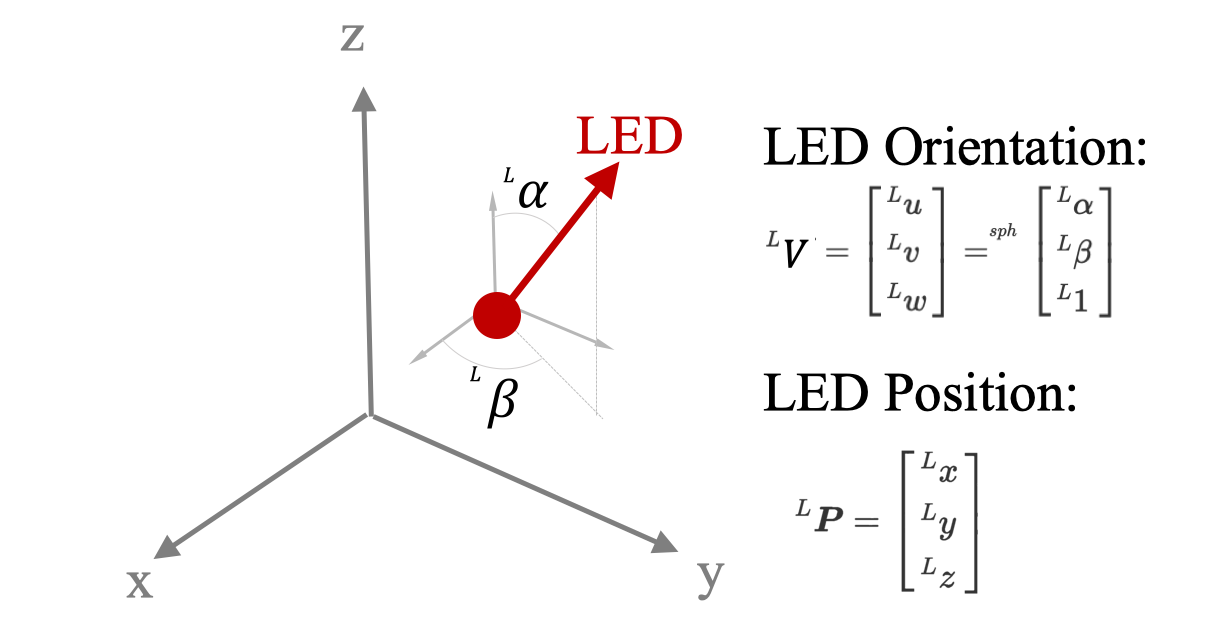
\includegraphics[width=10cm]{ch2pic/LED_config.png}
            \caption{LED在座標系中的擺放自由度}
            \label{pic:led_config}
        \end{figure}

        \qquad
        圖\ref{pic:led_config}以LED為例,呈現在空間中擺放的共五個自由度,而PD的擺放自由度相同。

        \item[- 將LED投影到PD座標系上]\hfill 
        
        \qquad

        \item[- 於PD座標系中計算距離、出入射角]\hfill 
        
        
        \qquad

    \end{description}   


        


















    \subsection{LED與PD定位現況與所遇困難}
    \label{chp:LEDPD_problem}



    


   

    


    

    

        
    

        




        
    以下分相探討此領域所欠缺的面向。
    
    \begin{description}

        \item[- 較少硬體實驗驗證]\hfill 
        
        \qquad
        在LED與PD系統中的研究,大多僅使用模型模擬,實際架設硬體進行實驗的案例較少,其中\cite{case:hypercube}\cite{case:3d_layers}為有進行硬體實驗的少數研究。

        \qquad
        模擬的研究中,大多研究會忽略各種誤差來源,其中最常被忽略的是多重路徑傳輸(圖\ref{pic:multipath})所產生的誤差,原因為多重路徑傳輸與環境、障礙物的位置相關,環境若時常出現變動,則需大量的模擬。除此之外,多重路徑傳輸的模擬難度高,愈複雜的環境、考量越多NLoS訊號,則需要更長的模擬時間。

        \item[- LED與PD的朗博次方被簡略]\hfill 
        
        \qquad
        朗博次方是一個影響輻射模式的重要參數(參考\ref{chp:lambertian}章),LED與PD兩者皆有各自的朗博次方,代表著訊號對角度敏感度與覆蓋範位的取捨。然而,大多研究皆將其省略,以便降低系統複雜度。
        
        \qquad
        將PD的朗博次方納入考量的文獻少之又少,相較起來,LED朗博次方有部分研究有將其納入計算,如\cite{case:cart2d}\cite{case:cart3d}。然而,假設朗博次方為一在實際上是不符合現實的,實際上在挑選硬體時朗博次方有許多選擇,為了降低複雜度而省略朗博次方,會侷限了能夠使用的硬體,也限制了系統的自由度。

        \item[- 缺乏三維定位的演算法]\hfill 
        
        \qquad

        \item[- 硬體組態自由度低]\hfill 
        
        \qquad
        同樣是為了降低系統複雜度,大多LED的組態為平行的等距陣列,有些類似於多點定位的擺法(參考圖\ref{pic:env_finger})。

        \qquad
        PD常見的組態類型為所有PD位於同一點,僅改變各PD的指向,如圖\ref{pic:config_orient},雖然指向能夠改變,大多情況仍會給予限制,例如所有PD的天頂角需相同等。

        \begin{figure}[ht]
            \centering
            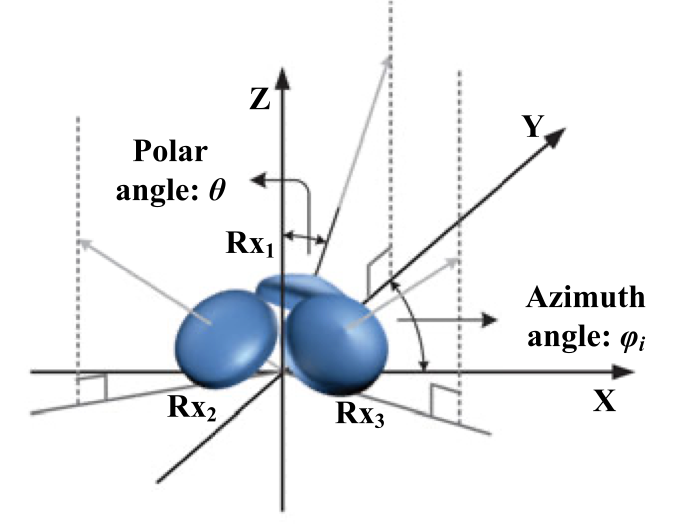
\includegraphics[width=6cm]{ch2pic/config_orient.png}
            \caption{常見的PD組態\cite{case:3d_layers}}
            \label{pic:config_orient}
        \end{figure}
        
        \item[- 限制使用情境]\hfill 
        
        \qquad



    \end{description}



    %     以下由硬體數量、使用情境限制、二維或是三維定位、朗博次方的考量、LED與PD的擺設方式等面向切入介紹與分析:

    %     \subsubsection{硬體數量}
    %     硬體數量上,大多是單個對多個的組合,單個LED對多個PD的方法\cite{case:cart2d}\cite{case:cart3d}\cite{case:3d_layers}優勢在於不用考量光的干涉,僅有單個光源連編碼解碼的部分也可以有條件的省略,簡化了系統複雜度。多個LED對單個PD的優勢則在於訊號處理不需同步多個PD,該PD進行解碼之後即可在計算單元內進行演算法的運作,不需綜合多個PD、考量到不同硬體時間的不同步,一樣簡化了系統複雜度。多對多的方法\cite{case:ml}雖然增加了系統複雜度,然而能獲取到的資訊同樣也較多。

    %     \subsubsection{硬體組態}   
    %     LED與PD的擺設方式上,為了降低\ref{eqn:model}所描述的模型複雜度,最常見到的LED擺設方式便為中心軸平行的等距陣列(補圖),PD擺設方式則是全部位於同個位置、同樣仰角,方位角則等距分配(補圖)\cite{case:cart2d}\cite{case:cart3d}\cite{case:3d_layers}。以上兩種最常見的擺設方式皆是為了降低系統複雜度,其中將PD擺放於同個位置僅改變指向,可使不同PD的距離與LED出射角這兩個變數一致,即可進行消除。
        
    %     \subsubsection{演算法}
    %     演算法上,如\ref{chp:method}介紹,常見的方法如多點定位、三角定位、指紋法,都需要有多個參考點,雖然多個參考點能夠提高精度,但是此種演算法裝設與事先校正都十分複雜,無法應對環境的改變,不符合不本論文研究目標的靈活應用。
        
    %     另一類型則是利用光傳遞模型\ref{eqn:model},利用模型變數為出入射角與距離三項幾何關係,推算出兩座標系的相對位置。此種演算法因為方程式的複雜度過高,使得需透過組態的限制來降低複雜度,例如限制擺設方式、或是使用情境的限制。

    %     常見的PD組態多限制各PD擺設於同點,僅能改變PD朝向,且朝向大多也會限制為同樣天頂角、或是限制指向多面體的頂點;常見的LED組態則是陣列存在,類似於室內空間中多個LED燈於天花板朝下照射的模式。

    %     使用情境則大多限制為「目標物與量測者需平行」,不得進行旋轉的移動,此限制雖然大大減少了系統複雜度,然而無法旋轉的使用情境過度受限,無論是人機互動,亦或是此類研究最常舉的案例:手機內鏡朝上於房間內走動,假設兩者僅能平行實在不合理,然而不限制平行的方法皆是使用多參考點的方式,現今仍沒有同時兼具不受旋轉影響又不需事先校正、安裝的方法,因此設計不受此限的演算法便是本研究主要目的之一。

    %   
    %     
        
    %    
    %     

        
    %     (不確定走向,所以先用列表整理在Notion之後確定再補上)
    %     % 補

    %     \begin{figure}[ht]
    %         \centering
    %         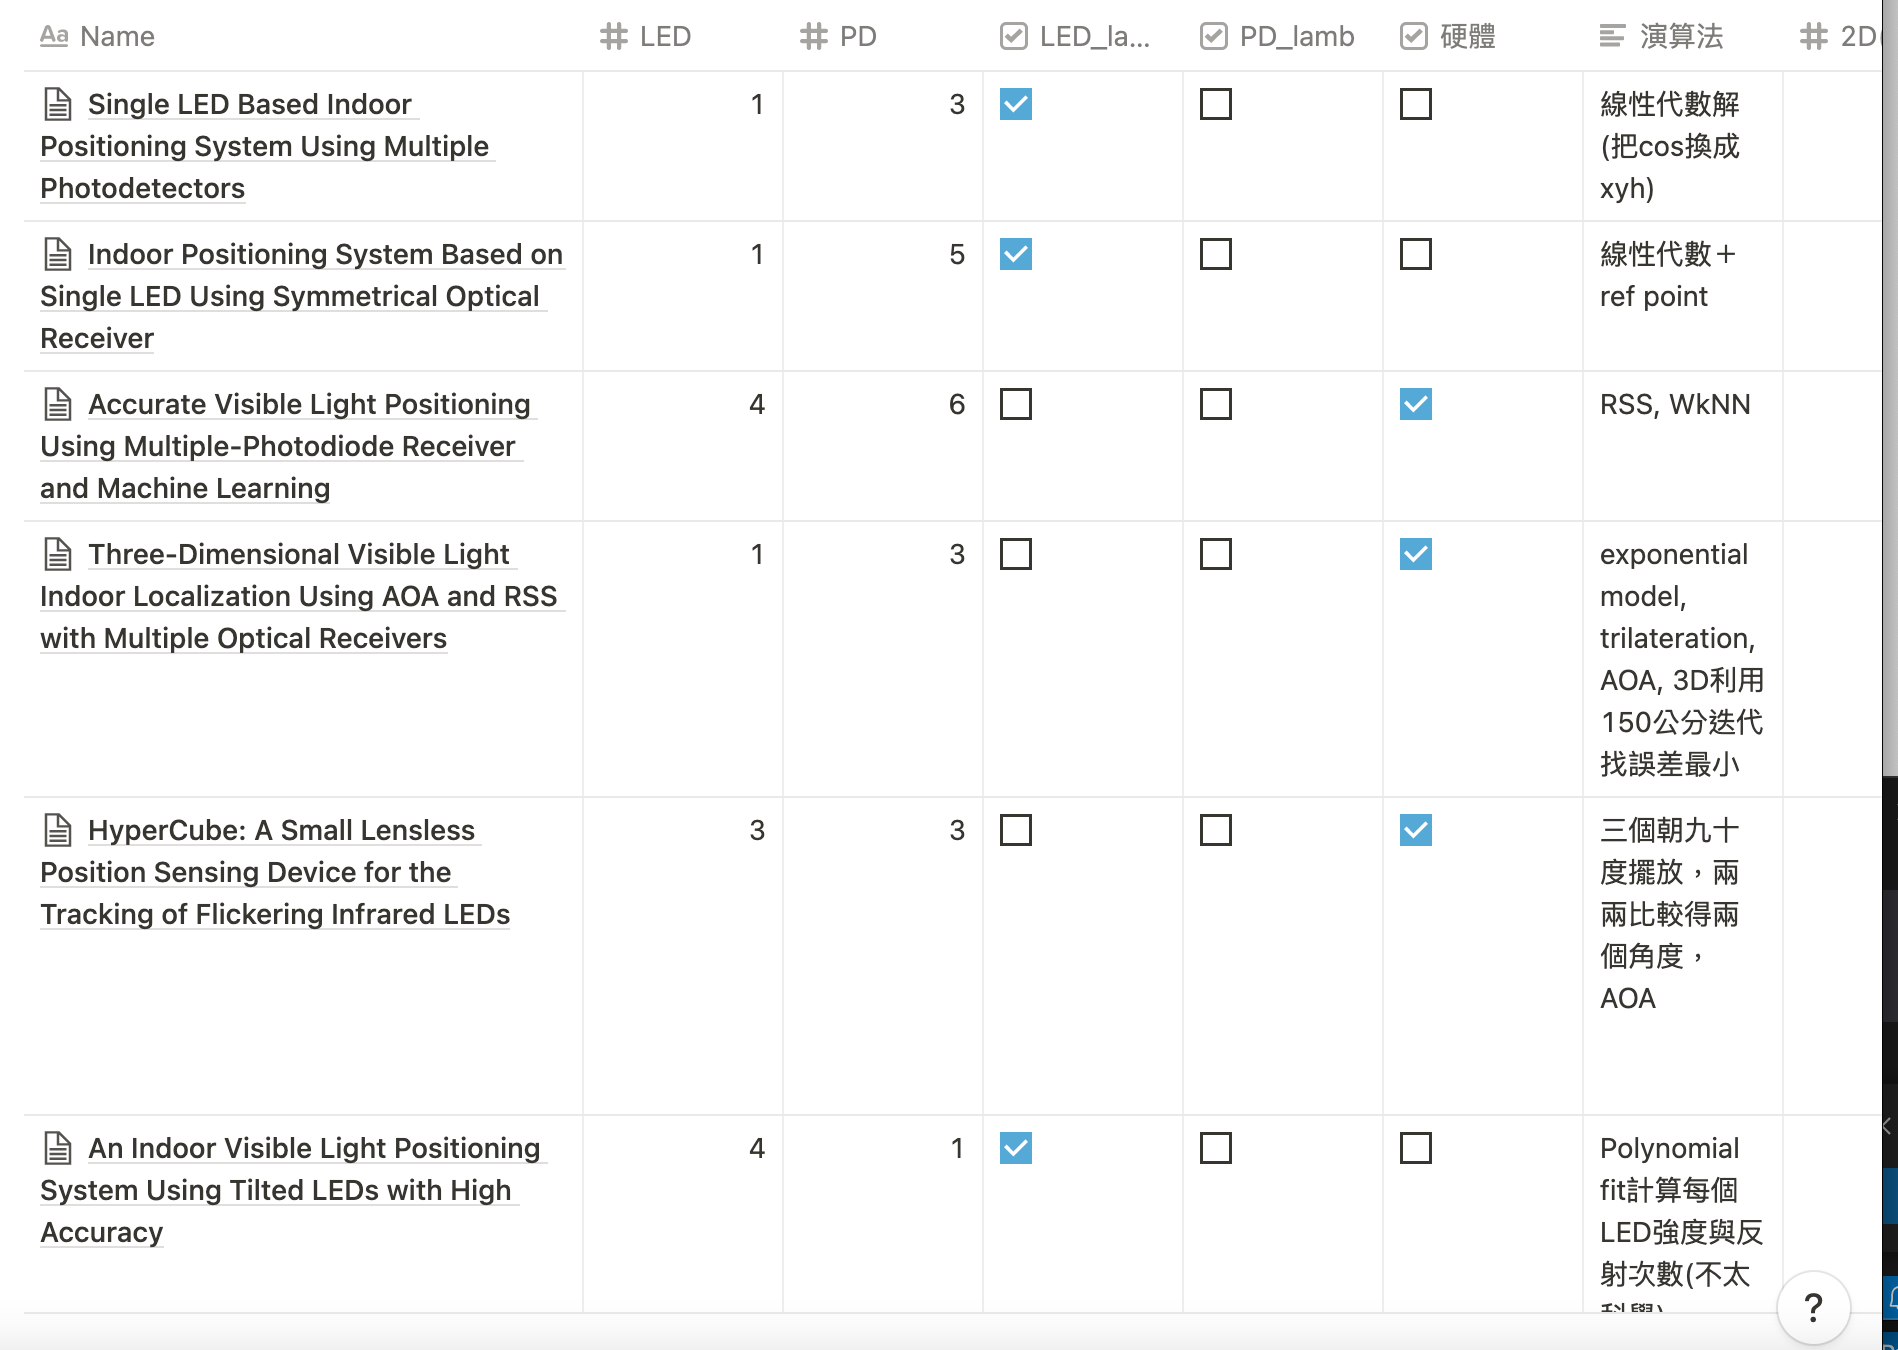
\includegraphics[width=10cm]{00temppic/temp.png}
    %         % \caption{多重路徑傳輸\cite{pic:multipath}}
    %         % \label{pic:multipath}
    %     \end{figure}



\section{結論}
\label{chp:2_conclusion}

利用LED與PD的技術,且使用幾何方法類型演算法的文獻,近年來開始被討論且具有靈活應用的潛力,然而此領域有以下不足:較少硬體實驗驗證、大多文獻忽略LED與PD的朗博次方,應用大多侷限在二維、硬體組態自由度低、且大多限制使用時目標物與量測者需平行。

本研究主要針對部分缺點進行改進,首先,本研究考量LED與PD的朗博次方,完整將硬體不同的輻射模式納入模型;另外,本研究於\ref{chp:3}章中提出一能夠達到三維定位,且不需限制目標物與量測者平行,大大增加了靈活度。

